\documentclass[10pt,twocolumn,letterpaper]{article}
\usepackage[T1]{fontenc}
\usepackage[review]{cvpr}
\usepackage{graphicx,amsmath,amssymb,booktabs,microtype,multirow}
\definecolor{oursteal}{HTML}{008C88}
\definecolor{cvprblue}{HTML}{176D89}
\PassOptionsToPackage{hyphens}{url}
\usepackage[pagebackref,breaklinks,colorlinks,allcolors=cvprblue]{hyperref}
\def\confName{CVPR}\def\confYear{2027}
\newcommand{\R}{\mathbb{R}}
\newcommand{\spn}{\operatorname{softplus}}
\newcommand{\tr}{\operatorname{tr}}
\newcommand{\dev}{\operatorname{dev}}
\newcommand{\diag}{\operatorname{diag}}
\newcommand{\file}[1]{{\small\nolinkurl{#1}}}
\title{Beyond Visual Agreement:\\Supplementary Material}
\author{Anonymous submission}
\setlength{\textfloatsep}{9pt plus 1pt minus 1pt}
\setlength{\dbltextfloatsep}{9pt plus 1pt minus 1pt}
\setlength{\intextsep}{7pt plus 1pt minus 1pt}
\begin{document}
\maketitle
\section{Scope and Reading Guide}
This supplement consolidates the complete protocols and result tables behind the main paper. The first part gives controlled mechanics, observability, additional observations, dynamic drops and all six coupled-scene families. The second part gives public SoftVT and real PhysTwin adapters, every fresh episode and every real transfer pair, including unsuccessful compatibility gates. The final part records a later conditional-flow diagnostic that was not promoted to replace the established predictors.

All studies retain their original cohorts and metric definitions. They are not combined into a single benchmark average or attributed to one shared implementation. Geometry and correspondences are supplied; material/force identifiability and causal raw-video reconstruction are not established. No prior prediction is changed by manuscript consolidation. Manuscript figures are generated from saved measurements; schematic method illustrations are labeled as such.

\paragraph{Implementation contract.}
Controlled six-family mechanics uses a frozen bulk decoder and quadratic supplied fixtures. The separate static inverse study uses both bulk and nonlinear attachment decoders. Real captured objects use tetrahedral equilibrium with the frozen bulk family and quadratic attachments. SoftVT uses analytic mechanics and a split pose/contact correction. These distinctions are essential when assigning a gain to a component.


\section{Adapter contracts and active physical laws}
\label{sec:adapter-contracts}
The experiments share a decomposition into material, tool-relative and
world-dependent terms. They do not share every law, state discretization or
inference procedure. Table~\ref{tab:adapter-contracts} summarizes the four
implementations. In particular, the nonlinear learned attachment law is used
in the static descriptor-refinement experiment, not in the headline six-family
coupled benchmark or the real-object adapter.

\begin{table*}[t]
\centering\small\setlength{\tabcolsep}{4pt}
\caption{\textbf{Which components are active?} All rows use supplied reference
geometry and correspondences. A frozen constitutive decoder is a material
prior; it is not a frozen scene-specific parameter estimate.}
\label{tab:adapter-contracts}
\begin{tabular}{p{.14\textwidth}p{.25\textwidth}p{.27\textwidth}p{.25\textwidth}}
\toprule
Study & Bulk and fitted descriptors & Attachments and environment & State evolution\\
\midrule
Six-family simulation & Frozen scalar energy; scale, volumetric multiplier,
spatial contrast and transition; second-body scale when present & Supplied
quadratic Gaussian/taper fixtures; explicit conservative normal penalties;
known density and collision geometry & Structured Q2 hexahedra, consistent
mass, velocity Verlet; coupled soft bodies and translating rigid sphere\\
Real PhysTwin & Frozen scalar energy; six material-field coefficients,
two global nonlinear descriptors and volumetric adjustment & Quadratic
prescribed-tool penalties; supplied footprints/activity, fitted strengths
and effective gravity/floor parameters & Filtered tetrahedral equilibrium;
implicit differentiation and bounded scene fitting\\
SoftVTBench & Analytic Neo-Hookean shape anchor and prefix-fitted corrections
& Tool-relative slip/release; known static environment & Equilibrium anchor
plus separate rigid pose/contact rollout; impulses do not deform the anchor\\
Static observation refinement & Frozen bulk and nonlinear attachment
energies; 15 continuous material/interface descriptors & Inferred attachment
strengths, nonlinearities and Gaussian footprint locations/widths; known
families, geometry, density and gravity & Structured Q2 equilibrium with
implicit sensitivities; separate reset commands\\
\bottomrule
\end{tabular}
\end{table*}

\paragraph{Six-family material and attachment laws.}
The pretrained bulk decoder is extended by an independently fitted positive
volumetric multiplier. With $B_\theta(s)$ denoting its original positive
volumetric coefficient,
\begin{equation}
 W_{\theta,\beta}(F,s)=W_\theta(F;s,0,-1)
 +(e^\beta-1)B_\theta(s)(J-\log J-1).
\end{equation}
The fitted field is
\begin{equation}
 s_b(X)=s_0+\mathbf{1}_{b=2}\Delta s+
 c\tanh\bigl(8(X_1-r)\bigr).
\end{equation}
There are four parameters $(s_0,\beta,c,r)$, with $\Delta s$ added for the
second body. The nonlinear descriptor coordinates are fixed at $(h,f)=(0,-1)$.
The same spatial parameterization is enabled in every family; the family name
does not supply the hidden material heterogeneity. No decoder weights are
updated during these fits.

For this benchmark, fixture energy is quadratic:
\begin{align}
 \Pi_b&=\frac12\alpha_b(t)K_b
 \int_{\Gamma_b}w_b(X)\|x(X)-T_b(X,t)\|^2\,dA_0,
 \nonumber\\
 &\int_{\Gamma_b}w_b\,dA_0=1.
\end{align}
The prescribed release gate $\alpha_b$ scales the assembled fixture matrix.
$K_b$ has units N/m; footprint normalization prevents it from becoming a
per-node stiffness that changes with mesh density. The force and actuator
work use derivatives of the same quadratic energy. The tested actuator
paths translate their fixtures; general rotating fixtures are not evaluated
in this six-family protocol. The older nonlinear attachment decoder is not
called by this rollout.

World contact uses a gap function and a conservative penalty. For the
parabolic bowl, the normalized implicit gap is an approximation to geometric
signed distance, rather than an exact Euclidean distance. The scene does
not implement friction, continuous collision detection or general rotating
rigid-body collision. A finite-mass sphere translates under equal-and-opposite
contact forces. Two deformable bodies retain separate material and state
variables. These capabilities do not imply discovery of contact topology
from images.

\paragraph{Real-object units and regularization.}
The real adapter normalizes coordinates by the initial bounding-box extent
and divides the pretrained bulk energy by its 12,000\,Pa reference energy
scale. It replaces the analytic bulk contribution while retaining the
external adapter's quadratic tool attachments, gravity and floor terms.
Its six Gaussian material features are distinct from the synthetic
$tanh$ field. The two global nonlinear descriptors and an independent
volumetric adjustment are optimized with the spatial field; network weights
remain frozen. Geometry filtering reduces tetrahedra bridging empty parts
of the reconstructed cloud, but does not certify a watertight physical
interior.

The inherited external energy includes a weak numerical reference-position
penalty $\tfrac12\epsilon\sum_i\|x_i-X_i\|^2$ with $\epsilon=10^{-5}$ in
normalized units. This regularization must not be interpreted as an inferred
physical fixture. Effective gravity/material and attachment/material ratios
are fitted; absolute real elastic moduli are not established by this
normalized position-only inverse problem. The first observed configuration
is treated as an effective rest shape, so unknown prestress remains a source
of model error.

\paragraph{Static nonlinear attachments and the scale argument.}
The separate static refinement study uses the learned nonlinear attachment
potential detailed below, with the quadratic spring recovered at zero
nonlinearity. Its unknowns include boundary footprint centers and widths;
that result cannot be reassigned to the known-boundary six-family study.
The exact common-scale ambiguity concerns an idealized energy in which
\emph{all} stiffness-bearing terms are co-scaled and independent body loading
is absent. It does not assert exact scale invariance for an external
implementation with an unscaled numerical reference pin or fixed contact
stiffness. Known gravitational or inertial scale information can break the
stated symmetry without guaranteeing global identifiability.

\part*{Controlled Mechanics and Physical Evaluation}

\section{Controlled-study map}
The controlled evidence comprises three earlier settings: (i) static composition with oracle physical descriptors, (ii) static inference of 15 continuous unknown descriptors and acquisition of an additional position observation, and (iii) dynamic calibration followed by larger-drop prediction against a native PhysTwin adaptation. A fourth study extends dynamic prediction to six coupled-scene families with unknown materials and known boundaries; its protocol is specified in Sec.~\ref{sim-sec:complex-scenes-supp}. Results from these settings are not interchangeable. In particular, the dynamic experiment does not evaluate the static active policy or its uncertainty model.

The central representation is a reusable, conditional \emph{energy law}. A small shared network maps physical descriptors to coefficients of invariant energy functions. A conventional mechanics solver combines this bulk law with attachment and contact potentials. Scene-specific inference estimates descriptors while the shared network weights remain frozen. Gaussian appearance is attached to material coordinates and transported by the resulting deformation. The system does not learn a direct image-to-force map, reconstruct unknown topology, or learn friction from video.

\paragraph{Units and metric conventions.}
Coordinates and tool translations are in metres; rotation vectors are in radians; force is in newtons; torque is in newton-metres. Bulk energy density is in pascals, total energy in joules, attachment stiffness in N/m, and normal-contact stiffness density in N/m$^3$. Static tables report \emph{coordinate} RMSE. Dynamic benchmark tables report \emph{point-vector} RMS, which is $\sqrt{3}$ times coordinate RMS for identical samples and weights. Numerical qualification thresholds remain in their originally declared coordinate convention.

\paragraph{What is shared.}
The bulk network is frozen across controlled objects and mechanical compositions. The bilateral-interface network is additionally active in the static composition and descriptor-refinement studies; the six-family dynamic study uses supplied quadratic fixtures. Reference geometry, material-coordinate fields, prescribed tool poses, gravity, and collision geometry enter the solver explicitly. Gravity is an external body load, rather than an output of the interface network. The dynamic drop study uses the shared bulk law and analytic normal contact; bilateral learned interfaces are evaluated in the static composition study, not covertly inserted into a free-body drop.

\paragraph{What is conventional.}
Invariant hyperelasticity, finite elements, sparse Newton solves, penalty contact, consistent mass, Verlet integration, implicit differentiation, and affine covariance transport are established ingredients. Our implementation combines them with shared conditional laws and auditable descriptor inference. We do not claim a new finite-element formulation, proof of polyconvexity, a general collision engine, or calibrated uncertainty.

\begin{figure}[t]
\centering
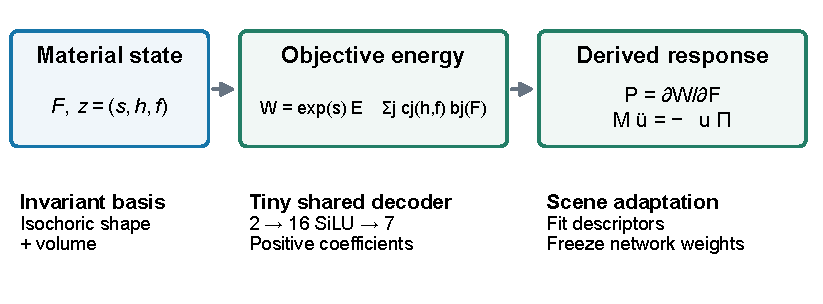
\includegraphics[width=\linewidth]{figures/sim-energy_block.pdf}
\caption{\textbf{Static learned-law composition.} This schematic depicts the bulk energy decoder; the separate nonlinear attachment decoder is specified in the text. The six-family and real-object adapters instead use quadratic attachments. Frozen constitutive weights are distinct from fitted scene descriptors and transported appearance.}
\label{sim-fig:energy-supp}
\end{figure}
\section{Conditional bulk energy}
Let $X$ be a material coordinate, $x(X)=X+u(X)$ the deformation, $F=\partial x/\partial X$, $J=\det F>0$, and $C=F^\top F$. Define
\begin{align}
 I_1&=\tr C, & I_2&=\tfrac12[(\tr C)^2-\tr(C^2)],\\
 q_1&=J^{-2/3}I_1-3, &q_2&=J^{-4/3}I_2-3,\\
 v(J)&=J-\log J-1.
\end{align}
The shared bulk energy is
\begin{equation}
 W_\theta(F;s,h,c)=e^s E_0\,a_\theta(h,c)^\top b(F),\qquad E_0=12000\ \mathrm{Pa},
\end{equation}
with
\begin{equation}
 b=[q_1/2,q_2/2,v,q_1^2,q_1^3,\phi_1(q_1),\phi_2(q_1)]^\top,
\end{equation}
\begin{align}
 a_\theta&=\spn(\mathrm{MLP}_\theta(h,c))+10^{-8},\\
 \phi_i(q)&=\spn(\alpha_iq)-\log2-\alpha_iq/2,\\
 \alpha_i&=\spn(\rho_i)+10^{-4}.
\end{align}
The coefficient decoder has two inputs, one 16-unit SiLU hidden layer, and seven outputs. Including the two slopes, it contains 169 parameters. The descriptor $s$ is a log common stiffness scale; $h$ controls nonlinear material shape; $c=-1$ and $+1$ designate the two teacher families. The scale enters only as $e^s$, not through the decoder. Spatial heterogeneity is represented through a material-coordinate descriptor field, rather than a separate network per object.

Objectivity and isotropy follow from the invariants. The reference energy and stress vanish at $F=I$. Stress $P=\partial W/\partial F$ and tangent $\partial P/\partial F$ are evaluated by automatic differentiation. Positive coefficients and reference normalization do not imply global convexity in $F$, uniqueness of equilibrium, or unconditional stability. The implementation rejects nonpositive determinants and applies additional sampled determinant guards during solves.

\section{Constitutive pretraining and interface laws}
\subsection{Bulk teachers and training}
The two analytic teacher families share small-strain moduli but differ at finite strain. With $a=\operatorname{sigmoid}(h)$, $\mu=4000e^s$ Pa, $K=20000e^s$ Pa, and $f=.15+.6a$,
\begin{align}
 W_{\rm MR}&=\frac{\mu}{2}[(1-f)q_1+fq_2]+Kv,\\
 W_{\rm Y}&=\mu\left[\tfrac12q_1+(.08+.3a)q_1^2\right.\nonumber\\
 &\hspace{32mm}\left.+(.01+.08a)q_1^3\right]+Kv.
\end{align}
These laws should not be confused with the separate stable-Neo-Hookean engine-control experiments.

Bulk pretraining uses 18 descriptor combinations: three scales $s\in\{-.5,0,.5\}$, three shapes $h\in\{-1,0,1\}$, and both families. There are 4096 training strain coupons and 512 validation coupons. Deformation gradients are upper triangular with log diagonal entries sampled in $[-.2,.2]$ and upper off-diagonal entries in $[-.4,.4]$. This supplies positive determinants. The objective is
\begin{equation}
\begin{aligned}
 \mathcal L_W={}&\operatorname{MSE}(P_\theta/12000,P_*/12000)\\
 &+.1\operatorname{MSE}(W_\theta/12000,W_*/12000).
\end{aligned}
\end{equation}
Training uses float64, batch size 256, 6000 fixed Adam steps, initial learning rate $.003$, and cosine decay. The final iterate is frozen before generating constitutive test coupons. No scene trajectories, reserved-object targets, or rendered future images are used to train this law. The tested interpolation descriptors use scales $\pm.25$ and shapes $\pm.5$; a harder strain test extends the log-diagonal/shear ranges to $.35/.7$.

\subsection{Nonlinear attachments in the static studies}
The following learned law is used for static composition and descriptor refinement. For a tool with reference origin $c_b$, translation $t_b$, and rotation $R_b$, define
\begin{equation}
 \delta_b(X)=x(X)-\{c_b+t_b+R_b(X-c_b)\}.
\end{equation}
The attachment is a bilateral compliant potential, not a unilateral collision constraint. Let $r=\|\delta\|^2/\ell^2$, with $\ell=.002$m. Its learned law is
\begin{equation}
 \psi_\theta(\delta;K,\chi,f)=\tfrac12K\ell^2\left[r+2\chi\sum_{j=1}^{7}a_j(\chi,f)\phi_j(r)\right].
\end{equation}
The bases comprise $r^2$ and six functions
\begin{equation}
 \phi_j(r)=\spn(b_j+\alpha_jr)-\spn(b_j)-\sigma(b_j)\alpha_jr.
\end{equation}
A two-input, 16-unit Tanh, seven-output decoder produces positive coefficients; six slopes and six offsets are also learned. There are 179 parameters. The outer stiffness factor is $K$, in N/m. At $\chi=0$ the interface is exactly quadratic. Tractions and tangents are derivatives of this scalar potential.

The analytic interface teachers use
\begin{equation}
 \psi_* =\tfrac12K\ell^2\{r+2\chi[(1-f)r^2+f(r-\log(1+r))]\},
\end{equation}
where $f=0$ is polynomial and $f=1$ is saturating in its nonlinear correction. The final wide-range checkpoint warm-starts the earlier small-slip model. Its 16384 coupons comprise equal numbers with radii up to $3\ell$ and $16\ell$, and strengths $.1,.3,.5,.7,.9$. Training uses 6000 fixed Adam steps, batch 512, initial learning rate $.003$, final rate $.0003$, and gradient clipping at 1. Force and energy residuals are normalized by $K\ell+\|t_*\|$ and $K\ell^2+|\psi_*|$, respectively, with energy weight $.05$. A failed wide-range random initialization remains recorded; it is not substituted into the final method.

\subsection{Spatial interface fields}
Attachment weights are reference-area weights multiplied by a Gaussian footprint and a smooth boundary taper, then normalized to sum to one. On normalized face coordinates $q=(q_y,q_z)$, the footprint is proportional to
\begin{equation}
 \prod_{d=y,z}4q_d(1-q_d)\exp\left[-\tfrac12\sum_{d=y,z}\left(\frac{q_d-c_d}{w_d}\right)^2\right].
\end{equation}
Centers $c_d$ and log-widths $\log w_d$ are fitted in the static inverse study and supplied in the six-family dynamic study. Normalization makes $K$ a total attachment stiffness rather than a mesh-dependent per-node constant. The weights are differentiable with respect to the centers and widths. Reactions and torques use the same integrated potential and current contact/attachment locations.

\paragraph{Scale ambiguity.}
For zero independent body load and fixed prescribed tool poses, multiplying all bulk and interface stiffnesses by $\alpha>0$ gives $\Pi_\alpha(u)=\alpha\Pi(u)$. Consequently the stationary and minimizing sets are unchanged, while reaction forces and tangents scale by $\alpha$. Position-only data cannot determine this common scale. This is a statement about a specified load model, not global identifiability. Known gravity or known-mass timed dynamics can break the symmetry. A contact term must also be co-scaled for this identity; fixed numerical contact compliance otherwise provides a relative scale.

\section{Forward solver, contact and motion}
\subsection{Controlled Q2 discretization}
In these controlled studies, the displacement field is interpolated with tensor-product quadratic hexahedral basis functions. Each element has 27 nodes, and the structured layout is $(4n,n,n)$ elements. Thus $n=2,3,4,6,8$ correspond to 425,1225,2673,8281,18785 nodes, respectively. The parameter $n$ is not the total number of elements per direction. Geometry maps support variations of length, width, depth, taper and arch; arbitrary topology is not inferred.

The discrete potential is
\begin{equation}
 \Pi(u)=\sum_q w_q W_\theta(F_q,z_q)+\sum_b\sum_{q\in b}\bar w_q\psi_\theta(\delta_q,z_b)+\Pi_c(u)-f_g^\top u.
\end{equation}
Reference-volume and reference-area quadrature are explicit. Static equilibria use sparse Newton iterations with a checked linear residual, descent check and Armijo backtracking. Tangents are energy derivatives. Determinants are checked at quadrature locations and element check points, including nodal locations; these sampled checks are not a global continuous-element positivity certificate. Continuation within a prescribed action improves equilibrium initialization without treating a sequence of unrelated probes as a physical dynamic trajectory.

\subsection{Unilateral normal contact}
For a known plane or sphere signed distance $g(x)$,
\begin{equation}
 \Pi_c=\frac12 k_c\int_{\Gamma_0}\min(g(x),0)^2\,dA_0.
\end{equation}
The surface points follow the current Q2 deformation, while the integration measure is reference area. The stiffness $k_c$ has units N/m$^3$. Contact forces and rigid-body reactions are derived from this potential and evaluated at matching positions, including the torque lever arm. The sphere-contact Hessian need not be positive semidefinite because of surface curvature. Penalty contact allows penetration; we report penetration and numerical sensitivity rather than claim exact nonpenetration. Neither friction nor adhesion is included in this controlled penalty-contact model; the separate SoftVT pose/contact adapter uses a Coulomb impulse cap.

The earlier static contact-transfer diagnostic combined both analytic teacher families and the frozen learned laws with this contact potential. Its 16 fine states yielded four passing family/method numerical qualification sets. This is evidence of composition for known descriptors and known collision geometry, not unknown-contact inference or general contact robustness. Tiny-patch sampling failures and earlier resolution failures remain in the development record.

\subsection{Controlled dynamic integration}
The controlled dynamic sequences use a consistent mass matrix,
\begin{equation}
 M_{ab}=\int_{\Omega_0}\rho N_aN_b\,dV_0,\qquad M\ddot u=-\nabla_u\Pi(u),
\end{equation}
and velocity Verlet: a half velocity update, position update, force recomputation, and second half velocity update. The mass matrix is factorized once. The controlled free-body scenes remove attachments exactly and have no weak reference anchor. This statement does not apply to the separately regularized external tetrahedral adapter. Gravity is a known body force. All dynamic videos sample actual integration states rather than interpolating static equilibria.

A separate finite-mass spherical striker stores center, velocity, angular velocity, mass, and spherical inertia. Its normal reaction is the opposite of that on the soft body. The current implementation is not a general rigid-scene collision engine: spherical orientation is immaterial to isotropic normal geometry, and not every rigid--rigid contact pair is supported. Momentum diagnostics use $Mv$, and angular momentum uses $\sum_a x_a\times(Mv)_a$.

The zero-damping drop benchmark is separate from the exploratory viscous tests. The latter use objective Kelvin--Voigt stress
\begin{align}
 D&=\operatorname{sym}(\nabla_XvF^{-1}),\\
 \sigma_v&=2\eta\dev D+\zeta\tr(D)I,\qquad P_v=J\sigma_vF^{-\top},
\end{align}
with $\eta=20$, $\zeta=40$ Pa\,s and a velocity-dependent explicit-midpoint integrator. Its dissipated power is nonnegative:
\begin{equation}
 \dot D_{\rm diss}=\int_{\Omega_0}J[2\eta\|\dev D\|^2+\zeta(\tr D)^2]dV_0.
\end{equation}
Both the material and integrator differ from the conservative control, so this is not an isolated causal damping ablation.

\subsection{Earlier drop-study appearance transport}
In the earlier four-world drop comparison, a canonical Gaussian is bound to a material coordinate $q$ with offset $r=\mu_0-X(q)$. At time $t$,
\begin{equation}
 \mu_t=X(q)+u_t(q)+F_t(q)r,\qquad \Sigma_t=F_t(q)\Sigma_0F_t(q)^\top.
\end{equation}
The covariance is refactorized into scale and rotation for rendering. The shared initial appearance checkpoint and opacity filter are used for both methods. Opacity and spherical-harmonic coefficients remain frozen; the returned polar material rotation is not applied to the SH coefficients. Native PhysTwin uses its author transport routine with $K=16$ neighbors, including its own scale/rotation behavior. Consequently image comparisons include both motion and transport differences. Initial canonical geometry is known, not recovered with COLMAP.

\section{Inference and static transfer evidence}
\subsection{Fifteen continuous unknowns}
The static unknown-physics experiment estimates bulk log-scale, shape and heterogeneity amplitude; left/right log-stiffness and nonlinear strength; four support-center coordinates; and four support log-widths. Geometry, material family, interface family, heterogeneity-pattern category, gravity and density are known. Therefore ``15 unknown descriptors'' does not mean unknown categorical discovery.

For observations $y$ at prescribed poses, the objective combines noise-normalized position residuals and a Gaussian descriptor prior. Implicit derivatives satisfy
\begin{equation}
 H\frac{\partial u}{\partial z}=-\frac{\partial R}{\partial z},\qquad H=\frac{\partial R}{\partial u}.
\end{equation}
Each parameter direction uses the same equilibrium factorization. Wrench derivatives, when used diagnostically, include both direct parameter dependence and the displacement derivative. The bounded trust-region reflective least-squares optimizer uses Jacobian scaling, a neutral initialization, at most 40 evaluations and 900s per fit. Numerical equilibrium, linear-system and tangent checks precede acceptance of derivatives. The unknown-action study uses position observations only; reaction forces are held predictions, not additional fitting observations.

\subsection{Oracle composition and geometry}
\begin{table}[t]
\centering\small
\begin{tabular}{lrr}
\toprule
Method & Composition & New geometry\\
\midrule
Matched analytic & .01642 & .01590\\
Neo-Hookean control & .02953 & .02982\\
Shared learned laws & .01811 & .01835\\
Custom direct, stable 6k & 3.65036 & 3.75043\\
Custom direct, stable 30k & 3.08880 & 3.29332\\
\bottomrule
\end{tabular}
\caption{Static oracle-descriptor transfer: displacement coordinate RMSE in mm. Each column contains six objects and four held commands per object. These are not results of unknown-descriptor inference.}
\label{sim-tab:oracle}
\end{table}
The withheld-composition cohort contains six objects. The geometry cohort contains six draws on two unseen geometry parameterizations of the same mapped-cuboid topology, with familiar categorical compositions; these are not six independently new geometry families. Predictions use $n=4$, references $n=8$, and 343 material queries. Coordinate RMSE is computed per command, then averaged over four commands and equally over objects. The shared model is close to matched analytic mechanics in this setting (Table~\ref{sim-tab:oracle}). Reference resolution was assessed in development; no per-reserved-object continuum certificate is implied.

The direct comparator is a custom DeepSets network, not a published MeshGraphNet implementation. It uses three 128-unit SiLU layers for each node/global encoder, mean and max node pooling, a displacement decoder with three 128-unit SiLU hidden layers and a linear output queried at material points, and a separate 12-output wrench head. Inputs include matched physical descriptors and frozen-law numerical fingerprints. Training uses 54 scenes with six actions each (324 records), and four validation scenes (24 records), with 125 input material nodes and 343 output queries. Its fixed 6k/30k training runs are retained.

The original direct normalization produced severe extrapolation from exactly zero training-feature columns. A separately declared stable-input control replaced only these zero-column scales by public physical units, leaving weights, targets, and nonconstant normalization unchanged. This control was motivated by training/public-input diagnosis, not selecting the best held prediction. The original results remain archived. A directory-only IO recovery later produced the stable-control artifacts after primary results had been visible; this operational history is disclosed rather than presenting a pristine single run.

\subsection{Additional observation and uncertainty}
\begin{table}[t]
\centering\small
\begin{tabular}{lrrr}
\toprule
Shared fitted policy & Pos. mm & Force N & Cov.\%\\
\midrule
Initial observations & .33949 & .09605 &97.01\\
Fixed stretch & .08022 & .02921 &33.01\\
Target-task variance & .08022 & .02921 &33.01\\
Fixed right bend & .21633 & .04278 & --\\
Fixed opposed twist & .08347 & .02851 & --\\
Seeded random & .09732 & .03429 & --\\
\bottomrule
\end{tabular}
\caption{Six fresh objects, two held commands per object. Position and force use coordinate RMSE. Cov. is nominal 90\% marginal position coverage for the primary local uncertainty approximation. Dashes denote values not tabulated here, not missing prediction attempts.}
\end{table}
The experiment observes 26 positions with 50$\mu$m coordinate noise and predicts two held command responses, using $n=2$ inference and $n=4$ references. It fits 48 unique models, of which 41 report optimizer success and seven retain incomplete-optimization forecasts. All 12 selected stretch refits converge. There are 144 complete scored rows across two model types, six policies, six objects and two commands.

The target-task variance policy chooses stretch on all six objects. Thus the improvement after one additional observation is real, but does not demonstrate adaptive superiority over a well-chosen fixed probe. The policy knows the target commands. Point accuracy improves while primary 90\% coverage falls sharply. Adding a separately frozen, validation-derived forward-discrepancy mean-square term expands intervals and raises coverage, but this is a supplementary predictive diagnostic: it does not refit likelihoods, change the policy or prove calibration. Model discrepancy at oracle descriptors need not cover inference bias.

\section{Fresh dynamic cohort and native comparison}
\subsection{Data and frozen fitting recipe}
Four fresh synthetic worlds use the known $0.12\times0.06\times0.06$m block and 0.27kg mass. Two worlds per analytic material family are shuffled into opaque identifiers. Private scale and shape are continuously sampled; contact stiffness is sampled log-uniformly between $2\times10^7$ and $8\times10^7$ N/m$^3$. Calibration is a 10mm-clearance drop for 0.20s. Forecasts are 40mm and 80mm drops for 0.30s, with gravity 9.8m/s$^2$, zero initial velocity and no friction. The reference and our model have no physical damping; native PhysTwin fits drag and dashpot parameters. This tests load-magnitude extrapolation, not new interaction types or geometry.

Both methods receive the same 21 calibration frames at 100Hz, 98 masked surface tracks and known initial geometry/mass. These are oracle 3D tracks with visibility, not tracks reconstructed from raw RGB. Known interior geometry supplies 27 additional initial points for the native particle graph. Private family, material parameters and forecast trajectories are inaccessible to fitting. Forecasts contain 31 saved frames. All predictions are committed before scoring against future targets.

Our dynamic fitting variables are $\xi=(s,h,\log k_c)$ and a binary family candidate. Bounds are $s\in[-1,1]$, $h\in[-2,2]$, $k_c\in[10^7,1.6\times10^8]$. The position objective is
\begin{equation}
 L(\xi)=\frac{1}{3|\Omega|}\sum_{(t,i)\in\Omega,\ t>0}\|x_\xi(X_i,t)-y_{ti}\|^2.
\end{equation}
The 54-candidate catalog spans three scales, three shapes, three contact stiffnesses and two families. Only verified forward trajectories are reused; visibility-weighted losses are recomputed separately for each world. Each family receives a 24-evaluation Powell stage at $n=2$, followed by 32 evaluations at $n=3$. The selected prediction uses the lowest-loss saved finite $n=3$ candidate across both families, not necessarily the optimizer's final iterate. The inference timestep is 50$\mu$s. One of 16 optimization stages reports convergence; the other 15 are budget-limited. Nevertheless all eight selected forecasts complete. Completion is not reported as parameter convergence or parameter correctness.

\subsection{Native implementation and controls}
The native PhysTwin adaptation retains its spring-mass graph, optimizer and prediction routines. Development calibration selected the globally fixed 125-particle extended recipe: at most 100 CMA generations with the author implementation's early stopping, and 1000 epochs. A 729-particle capacity control was also evaluated in development using the same observed tracks and extra known initial geometry. No per-test-world recipe selection is performed. The native model has a different mechanical representation, discretization, contact parameterization and numerical dissipation; it does not receive our analytic teacher law.

The initial native orchestration failed because the child environment did not explicitly satisfy its GPU0 guard. No optimization from that failed attempt was treated as a valid result. An independently reviewed operational recovery used separate output directories and explicit environment settings, preserving the original failures, model recipe and frozen public inputs. The recovery completes three world fits and six forecasts. World 3 remains unavailable; it is not replaced by a new world or assigned an invented error.

\begin{table}[t]
\centering\small
\begin{tabular}{ccrrrr}
\toprule
World & Drop & \multicolumn{2}{c}{World RMS} & \multicolumn{2}{c}{Shape RMS}\\
& mm & Ours & Native & Ours & Native\\
\midrule
0&40&.9434&8.8154&.8581&2.4369\\
0&80&1.1800&19.4244&1.0652&2.8790\\
1&40&1.1501&8.5297&1.1296&3.2741\\
1&80&1.4850&17.7201&1.4616&3.7512\\
2&40&.9680&8.8291&.8928&2.3549\\
2&80&1.1510&19.3087&1.1050&2.9182\\
3&40&.8195&Failed&.7987&Failed\\
3&80&1.0098&Failed&.9623&Failed\\
\midrule
\multicolumn{2}{l}{Paired six only}&1.1462&13.7712&1.0854&2.9357\\
\bottomrule
\end{tabular}
\caption{Every fresh forecast attempt. Errors are point-vector RMS in mm, with fixed surface weights; shape removes one proper rigid transformation per frame. Native coverage is6/8, ours8/8. The paired row excludes both methods' world3 scores and is conditional on three completed native fits.}
\label{sim-tab:fresh}
\end{table}

The result is a controlled synthetic comparison to an adapted native method, not an official PhysTwin benchmark score or a broad SOTA claim. Analytic reference generation is closer to our model class than to a spring network. That advantage is part of the experimental design and limits generalization of the ranking. The native representation's scale and energy dissipation cannot be inferred from our continuum parameters alone.

\section{Reference sensitivity, rendering and failures}
\subsection{Finite-resolution reference assessment}
All 20 declared reference jobs complete and pass their individual trajectory checks. The primary generator is $n=4$, $\Delta t=25\mu$s. The fixed subset consists of one world from each family (worlds 0 and1), each with $n=6$ calibration and 80mm forecast companions and half-step80mm runs at both resolutions. These are finite-resolution analytic references, not continuum ground truth.

\begin{table}[t]
\centering\small
\begin{tabular}{clrrc}
\toprule
World & Comparison & World & Shape & Pass\\
\midrule
0&Calib. $n4/n6$ &.2235&.1813&No\\
0&80mm $n4/n6$ &.6162&.4198&No\\
1&Calib. $n4/n6$ &.2028&.1897&No\\
1&80mm $n4/n6$ &.7275&.4958&No\\
0&80mm $n4$ time &.00987&.00985&Yes\\
0&80mm $n6$ time &.02032&.02004&Yes\\
1&80mm $n4$ time &.01876&.01755&Yes\\
1&80mm $n6$ time &.02613&.02547&Yes\\
\bottomrule
\end{tabular}
\caption{All eight fixed-subset sensitivity comparisons, coordinate RMS in mm. Time compares 25 to 12.5$\mu$s. Common $6\times17\times17$ face samples and all saved frames are used. The world/shape thresholds are 0.300/0.150mm; all four spatial comparisons fail and all four temporal comparisons pass.}
\end{table}
The sampling norm in this qualification is a uniform face-sample coordinate norm, not an exact mass integral and not the 98-point benchmark weighting. Failure is retained rather than selecting an earlier passing mesh pair or relaxing thresholds. The initial sensitivity writer encountered a NumPy scalar JSON-serialization error; an additive scalar-conversion wrapper produced the report without changing any metric or selected record.

\begin{table}[t]
\centering\small
\begin{tabular}{clrrrr}
\toprule
World& Reference &\multicolumn{2}{c}{World RMS}&\multicolumn{2}{c}{Shape RMS}\\
&&Ours&Native&Ours&Native\\
\midrule
0&$n4$&1.180&19.424&1.065&2.879\\
0&$n6$&1.690&18.779&1.059&2.858\\
0&$n6$, half step&1.697&18.771&1.059&2.857\\
1&$n4$&1.485&17.720&1.462&3.751\\
1&$n6$&1.660&17.005&1.444&3.658\\
1&$n6$, half step&1.659&17.011&1.446&3.659\\
\bottomrule
\end{tabular}
\caption{Explicitly post-hoc secondary robustness check on the two already fixed 80mm cases. Frozen predictions are unchanged. Point-vector RMS in mm. The ranking persists, but the spatial reference failure is not thereby repaired.}
\end{table}

\subsection{Appearance and image metrics}
The same initial Gaussian appearance is fitted and frozen for both methods; no future images optimize physical predictions or appearance. The image pipeline seals all 2480 declared image slots before reference scoring: 2170 images are scored, and 310 native slots are missing and explicitly retained as failures. On the three paired completed worlds, held-image foreground-union PSNR is 18.734dB versus 12.842dB, foreground-union SSIM is .7473 versus .5770, silhouette IoU is .9562 versus .7950, and jointly visible depth RMSE is 5.478 versus 14.557mm (ours versus native). These are conditional three-world means, not an all-four paired estimate. Shared appearance reduces one source of confounding; different physical trajectories and different transport routines still contribute jointly.

\subsection{Development failures and qualified scope}
The abrupt 20\% compressed release remains spatially unqualified even after its bounded refinement ladder. More aggressive conservative releases and drops can encounter determinant guards; their available prefixes and termination reasons are retained. Energy conservation alone does not guarantee element validity. No artificial restitution or relaxed determinant threshold was introduced to make a failed drop look successful.

A separate smooth position-controlled compression/hold/unload reaches approximately 22.7\% actual end-face closure under 30\% commanded tool-separation change. Its $n3/n4$ world-coordinate discrepancy is 53.2$\mu$m and the declared joint checks pass. A smaller conservative drop passes its $n6/n8$ development checks, whereas that result is not inherited by the fresh material cohort. The viscous 40mm drop and a separate viscous striker pass their timestep pair checks but remain without spatial qualification. The displayed conservative 80g striker is a single-step-size demonstration, without that temporal qualification. Static learned-contact composition has its own qualified sets. These distinct statuses must not be merged into one universal ``physics validated'' label.

\section{Reproducibility, evidence and media}
\subsection{Source and artifact map}
The implementation separates bulk pretraining, interface pretraining, forward mechanics, descriptor inference, and rendering. The following filenames identify the source entry points; they are not additional experimental variants.

\begin{itemize}
\item Bulk invariants and basis: \file{materials.py}; exact common-scale wrapper: \file{scale_separated_material.py}; final pretraining: \file{train_scale_separated_material.py}.
\item Bilateral law: \file{interfaces.py}; final wide-range training: \file{train_interface_range_warm.py}; Q2 assembly and differentiable footprints: \file{mechanics.py}.
\item Normal contact: \file{contact_mechanics.py}; dynamics: \file{dynamics.py}; separate viscous variant: \file{viscous.py}.
\item Static inference: \file{joint_inference.py} and \file{gauss_newton_inference.py}; fresh dynamic inference: \file{cohort_shared_fit.py} and \file{matched_material_fit.py}.
\item Gaussian material transport: \file{gaussian_transport.py}; appearance adaptation: \file{cohort_appearance_transport.py}; native-author rendering bridge: \file{matched_gaussian_states.py}.
\end{itemize}
The first group resides in the compositional neural-mechanics source package; the dynamic experiment and cohort orchestration reside in the compositional-dynamics source package. Earlier frozen sources and reports are preserved rather than overwritten by recovery implementations.

\subsection{Evidence records}
Static oracle transfer is summarized in \file{oracle-recovered-plus-stable-io-comparison.json}. Its completed analytic/learned oracle artifact recovery passes 3822 independent checks, and the stable-input direct control passes 3570. These checks verify recorded artifacts and calculations, not a new theoretical correctness guarantee.

The unknown-parameter experiment is summarized in \file{unknown-action-reaction-paper-summary.json}, with separate action and reaction audits (931 and 1734 checks). The small conditional posterior studies and their recovery histories are distinct from the 15D local uncertainty approximation. Numerical consistency of a small reference posterior does not certify the larger inferred posterior or the dynamic benchmark.

Fresh dynamic scoring is recorded in \file{fresh-cohort-geometry-recovery-results.json}. Its independent audit checks 2686 identities, arrays and calculations. Reference sensitivity and post-hoc ranking checks are in \file{fresh-cohort-reference-sensitivity.json} and \file{fresh-cohort-reference-robustness-posthoc.json}, with 359 and 171 independent checks, respectively. Image results and conditional paired summaries are in \file{fresh-cohort-appearance-results.json} and \file{fresh-cohort-appearance-paired-summary.json}.

\paragraph{Sealing and recovery.}
The cohort protocol and source freeze precede private-world generation. Public calibration export binds world identity, protocol identity, observation arrays and metadata. Predictor processes receive public calibration and known forecast setups, not private material labels or future target arrays. Forecast commits include completion or failure and artifact digests. Geometry scoring waits for all original and recovery prediction slots; image scoring additionally waits for prediction-image commitments. Failures remain in cohort denominators. The native environment recovery, direct-baseline IO recovery and scalar serialization wrapper are operational amendments with separate records; none selects a better prediction using held targets.

\paragraph{Budget and precision.}
Constitutive derivatives and the Q2 mechanics path use float64. Resource limits terminate jobs with explicit incomplete records; optimizer iteration limits and trajectory completion are reported separately. A runtime success flag is not a convergence certificate. Shared law checkpoints are fixed during object fitting. Reproducing the full numerical evidence requires the pinned sources, checkpoints, canonical geometry, protocol files and local raw trajectory artifacts; the manuscript alone does not replace these inputs.

\subsection{Video inventory and interpretation}
The archived four-world dynamic comparison contains the following eight files
\begin{center}
\small\ttfamily
world-0-forecast-40mm-held0.mp4\\
world-0-forecast-80mm-held0.mp4\\
world-1-forecast-40mm-held0.mp4\\
world-1-forecast-80mm-held0.mp4\\
world-2-forecast-40mm-held0.mp4\\
world-2-forecast-80mm-held0.mp4\\
world-3-forecast-40mm-held0.mp4\\
world-3-forecast-80mm-held0.mp4
\end{center}
They use synchronized physical times and a fixed held camera. The filename world identifier is opaque and does not encode material labels. Failed native slots are explicitly indicated rather than filled with an apparently successful synthetic motion. These eight forecast clips and the four development clips below constitute the earlier twelve-clip media set; the six-family clips form a separate set described later. Reference and prediction clips display the finite-resolution benchmark, not captured real-world footage.

The four additional development clips are
\begin{center}
\small\ttfamily
position-compression-development.mp4\\
finite-striker-development.mp4\\
drop-bounce-settle-development.mp4\\
development-orbit-actual-ours-native-v2.mp4
\end{center}
These development clips are not additional held-cohort successes. Dynamic compression, drop and striker clips use sampled integrated states. No static-contact orbit clip is part of that earlier twelve-clip set. Slow playback changes presentation time, not the simulated physical timestep. Visual appeal, image fidelity and mechanical accuracy are reported separately.

\subsection{Interpretation of the earlier controlled studies}
The oracle study supports composition of reusable learned laws when physical descriptors are supplied. The unknown-descriptor study shows improved point predictions after an informative additional position observation, while exposing overconfident uncertainty and no advantage over its best fixed probe. The fresh dynamic study supports a conditional improvement over one native adaptation on synthetic load-magnitude extrapolation, with incomplete native coverage and unresolved spatial-reference sensitivity. These controlled findings do not themselves establish real-world transfer; the separate real-capture pilot below addresses that question on two compatible pairs. They also do not establish raw-video physical inference, unknown interaction discovery, general frictional dynamics or superior active probing.
\begin{figure*}[t]
\centering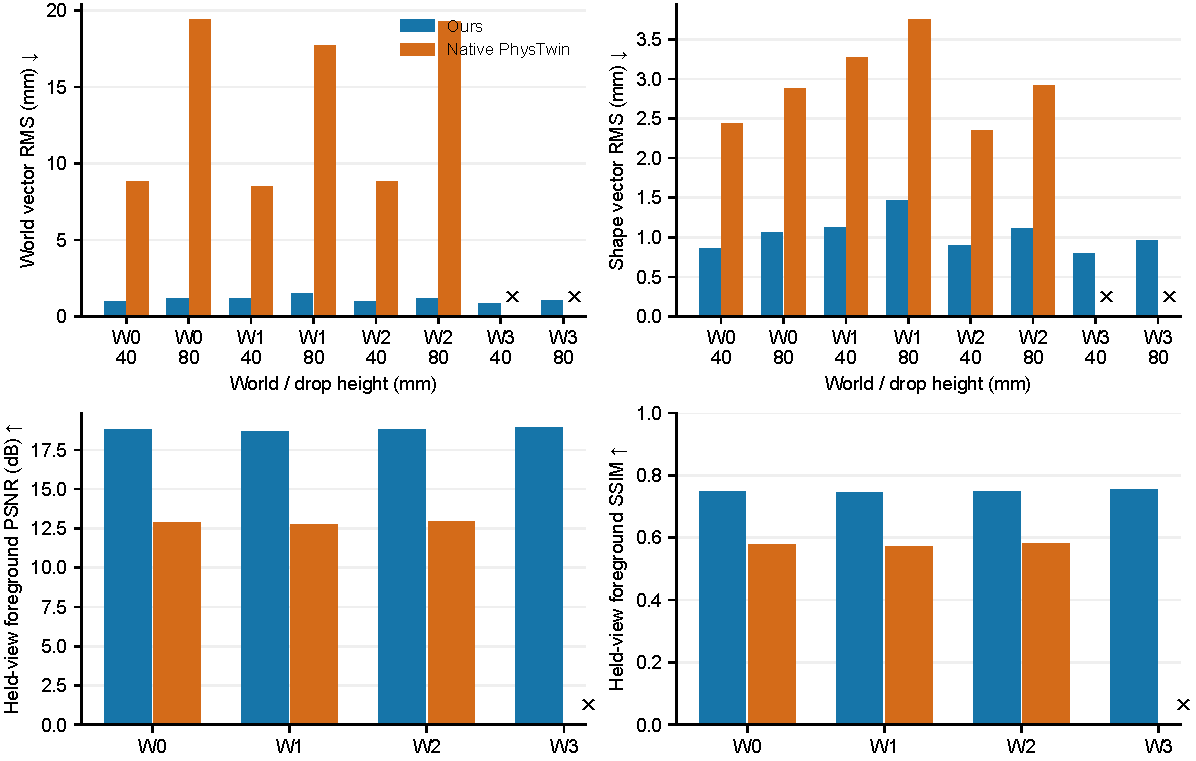
\includegraphics[width=.84\textwidth]{figures/sim-dynamic_results.pdf}
\caption{\textbf{All eight earlier drop forecasts.} Top: world and rigid-aligned shape errors for both forecast heights in each world. Bottom: held-view image metrics by world. Crosses mark unavailable native predictions in world 3; they are not zero-valued measurements. Shared appearance initialization makes the image comparison a test of predicted motion plus Gaussian transport.}
\label{sim-fig:dynamics}
\end{figure*}

\subsection{Earlier drop-cohort appearance illustration}
Figure~\ref{sim-fig:qualitative} illustrates the earlier four-world drop study; the six-family experiment below uses a separate held cohort.
\begin{figure*}[t]
\centering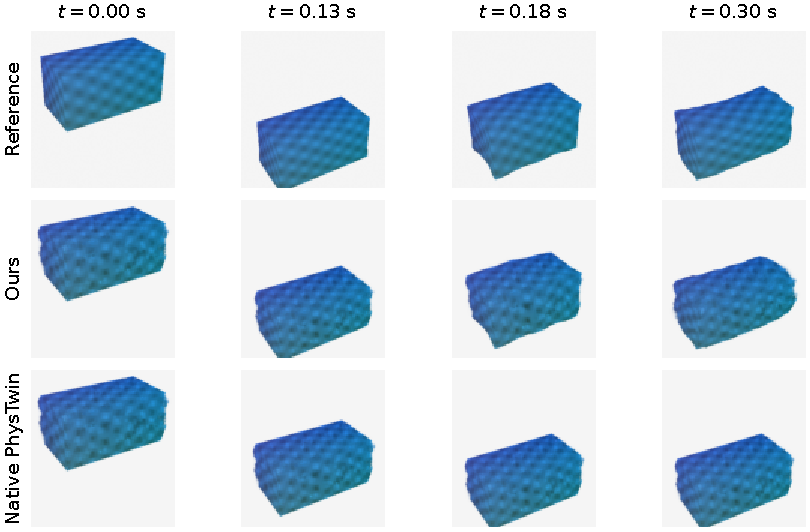
\includegraphics[width=.80\textwidth]{figures/sim-qualitative.pdf}
\caption{\textbf{Earlier four-world drop cohort: reference versus predicted appearance.} First declared world, 80\,mm forecast, first held camera. The same crop is computed across all methods and all 31 frames; RGB values are unchanged. Columns show 0, 0.13, 0.18 and 0.30\,s. This selection is a fixed case illustration, not an aggregate result. Some objects intersect the lower edge of the original saved camera viewport: reference/ours at 0.13\,s and native at 0.18/0.30\,s. No pixels are extrapolated.}
\label{sim-fig:qualitative}
\end{figure*}

\section{Six-family coupled-scene benchmark}
\label{sim-sec:complex-scenes-supp}
\subsection{Coupled-scene prediction protocol}
\label{sec:coupled-protocol}
We separate the material of an object from the interaction applied to it.
A world $w$ specifies fixed object geometry, density, and a hidden material
field $m_w$. An interaction $a$ specifies the initial state, prescribed fixture
positions and release schedule, gravity, and collision geometry. For each
world, a short calibration interaction provides point observations
$\mathcal D_w=\{(t_i,X_j,x_{ij})\}$ up to a fixed cutoff. A method fits its
material representation to this prefix, seals the fitted parameters, and
predicts two different interactions without refitting. The same hidden
material is retained across calibration and both queries.

The protocol contains six scene families: moving and released compliant
clamps; pushing around a curved obstacle; gravity drops into a curved
container, including an obstacle; a translating finite-mass rigid striker;
two deformable objects in collision or stacking; and spatially heterogeneous
material. Query changes include fixture location, displacement amplitude,
impact velocity, drop height and orientation, and contact configuration.
The frozen census is four independently sampled material worlds per
family and two queries per world. Object shape and density are fixed in
this study; transfer is across material and interaction, rather than unseen
object geometry.
The protocol, implementation inventory, model checkpoints, and development
decision were fixed before generating the held worlds. Young's modulus is
sampled log-uniformly from $8$ to $18$\,kPa and Poisson's ratio uniformly
from $0.25$ to $0.40$. Two-body scenes use independent material draws.
Heterogeneous worlds additionally sample a log-contrast corresponding to
factors between two and three and a transition coordinate between $0.35$
and $0.65$. These draws remain fixed across each world's three interactions.

All methods receive the same calibration tracks, rest geometry, density,
and public boundary parameters. Tracks cover a fixed two-face material-point
subset and are sampled every $2$\,ms. This controlled track-input study does
not measure image tracking errors or camera-dependent occlusion. Materials
are unknown, while fixture compliance and collision geometry are known.
Consequently, this experiment evaluates prediction conditional on supplied
boundaries; it is not an evaluation of unknown-boundary recovery.

\subsection{Shared neural material with spatial descriptors}
The pretrained energy decoder is kept fixed. We infer a small spatial
material descriptor from the calibration prefix. For material coordinate
$X\in[0,1]^3$, the scale field is
\begin{equation}
 s_b(X)=s_0+\mathbf{1}_{b=2}\Delta s+
 c\tanh\!\left(8(X_1-r)\right),
\end{equation}
where $b$ indexes the deformable body. The same field parameterization is
available in every family; the heterogeneous-scene label does not switch
on a privileged material model. A second body receives an additional scale
offset, while the spatial profile and compressibility parameter are shared.
The other two pretrained descriptor coordinates are fixed at their
values $(0,-1)$ in this experiment.

We extend the frozen decoder with an independent positive multiplier on
its volumetric contribution. Writing $W_\theta$ for the pretrained energy,
$J=\det F$, and $B_\theta(s)$ for its existing positive volumetric
coefficient, the extension is
\begin{equation}
 W_{\theta,\beta}(F,s)=W_\theta(F,s)
 +(e^\beta-1)B_\theta(s)(J-\log J-1).
\end{equation}
Thus $\beta=0$ recovers the previous model exactly. The descriptor parameters
are fitted by bounded derivative-free optimization of the observed
point-position loss. No network weights are updated on a held world.
Additional calibration stages, when selected in development, initialize
from the preceding sealed best fit to the identical observation prefix.
This changes the optimization budget without reading the future query.
The frozen schedule permits $64$ objective evaluations followed by up to
$128$ additional evaluations, initialized from the best calibration fit.
The analytic control receives the identical schedule. The best calibration
loss determines the parameters used for both queries; no query-specific
parameter selection is performed. Reaching an evaluation limit is reported
separately from optimizer convergence.

Predicted motion follows the coupled mechanics rollout with explicit
collision geometry and compliant fixtures. The current scene model includes
conservative penalty contact, separation, and translation of the rigid
sphere; it does not model general rotating rigid shapes, friction, or
continuous collision detection. These limits define the evaluated scene
capabilities rather than being hidden in an aggregate score.

\subsection{Adapted mechanics baselines}
We compare with PhysTwin~\cite{jiang2025phystwin},
Spring-Gaus~\cite{zhong2024springgaus}, and
UniPhy~\cite{mittal2025uniphy}, using pinned author implementations.
PhysTwin uses the author Warp spring-force kernel and native forecast
integration, with per-edge stiffness fitted to the common track prefix.
Spring-Gaus uses the author internal forces and integration, a scalar
stiffness initialization search, and subsequent per-edge fitting. Both use
known object masses and explicit common scene-boundary adapters. PhysTwin
uses fixed zero dashpot and drag damping in this adapter. These are
mechanics comparisons with disclosed interfaces, not reproductions of the
complete author image-reconstruction pipelines.
Both native spring adapters use $40$ Adam iterations with learning rate
$0.03$ and a four-hour fitting limit. Spring-Gaus first searches a scalar
stiffness initialization. Single-clamp development controls at $160$
iterations improved calibration but increased vector forecast error for
both adapters; these controls and their shape errors are retained alongside
the selected budgets. This observation does not establish that $40$
iterations is optimal for every scene. Actual successful iterations and
numerical failures are reported rather than assumed from requested budgets.

UniPhy uses the released pretrained constitutive networks and native MPM,
with a fitted material latent and explicit bowl/obstacle hooks. Its current
adapter supports the drop family only. Its native separating-velocity
projection differs from the conservative penalty contact of the reference
and the other adapters; its results therefore measure this adapted
system's capability, not a matched-contact-law material-inference error.
Any adjoint adaptation and its derivative checks are reported separately.
Unsupported configurations are retained as unsupported, rather than being
counted as failures or wins. An analytic Neo-Hookean control uses the same
spatial fitting parameterization but has the advantage of knowing the
reference constitutive family.
UniPhy uses eight fixed-seed latent-centroid initializations followed by
eight AdamW iterations at learning rate $3\times10^{-5}$. Its derivative
qualification remains coordinate-sensitive, which limits attribution of
any adapted-system failure to the original method.

\subsection{Physical and visual evaluation}
We report full-query point-position RMS and per-object rigid-aligned shape
RMS separately. Additional physical diagnostics include sampled contact
penetration and first-contact time, net nongravitational body impulse,
and signed tetrahedron-volume ratios on the same material grid for all
methods. The impulse is computed from saved velocity and known mass after
subtracting gravity; it does not resolve individual contact forces.
Sampled orientation and gap checks are diagnostics, not proofs of global
injectivity or continuous nonintersection.

For a controlled image comparison, every method and the reference use the
same frozen Gaussian appearance, the same motion-transport map, and fixed
withheld cameras. We report PSNR, SSIM, LPIPS, and silhouette IoU, averaging
noninitial query frames for the primary scores and retaining all-frame
values separately.
This separates motion-induced image error from independent appearance
optimization. The rendering is object-only and does not test environmental
occlusion or native end-to-end reconstruction quality. Image agreement and
physical agreement are evaluated separately; neither is inferred from the
other.

Numerical reference uncertainty is assessed through spatial refinement,
with dense sampled orientation checks. A completed reference trajectory is
not automatically treated as spatially converged. Fitting, rollout,
reference and infrastructure failures remain separately visible in the
complete planned census. We average the two queries within each world,
then compute paired method differences and bootstrap intervals by resampling
worlds, not frames. Error comparisons conditional on successful paired
worlds are accompanied by their completion and coverage counts.
References use Q2 meshes with $(4n,n,n)$ cells, $n=4$, Lobatto-4 quadrature,
and a $25$\,$\mu$s time step. Both queries of the preselected first world
in every family are repeated at $n=6$. These twelve comparisons quantify
resolution sensitivity on those worlds; they are not rigorous error bounds
or a population-wide convergence certificate. Our material model and the
analytic control use $n=1$ with $50$\,$\mu$s steps. Native spring adapters
use $25$\,$\mu$s steps and UniPhy uses $50$\,$\mu$s steps.

\subsection{Held physical prediction results}
\label{sec:coupled-physical-results}
Ours, the analytic control, Spring-Gaus and PhysTwin each complete all
48 held queries. Table~\ref{tab:coupled-physical} summarizes full-query
motion errors, including the shared initial frame, and rigid-aligned shape
errors. The paired mean motion-error difference across 24 independent
worlds is $-8.83$\,mm against PhysTwin (world-bootstrap 95\% interval
$[-12.18,-5.83]$) and $-9.30$\,mm against Spring-Gaus
($[-12.40,-6.50]$). Our difference from the analytic control is
$+0.13$\,mm ($[-0.01,0.27]$); this does not establish an advantage over
the matched analytic family. The analytic control knows the reference
constitutive family but fits its unknown material parameters from the same
observed prefix.

\begin{table}[t]
\centering\small
\caption{Six-family held physical prediction. Motion and rigid-aligned
shape RMS are in mm. Folds counts queries with any nonpositive sampled
material-grid tetrahedron volume; this is a common diagnostic, not a
continuous-injectivity certificate. All rows complete 48/48 queries.}
\label{tab:coupled-physical}
\begin{tabular}{lrrr}
\toprule Method & Motion & Shape & Folds \\
\midrule
Ours & 1.97 & 1.25 & 0 \\
Analytic control & 1.84 & 1.16 & 0 \\
PhysTwin adaptation & 10.80 & 5.94 & 33 \\
Spring-Gaus adaptation & 11.27 & 6.00 & 37 \\
\bottomrule
\end{tabular}
\end{table}

Our mean motion error is lower than both native adaptations in each of
the six families. Against the analytic control, our descriptive mean is
lower for clamps/release, curved pushing, two-body interaction and
heterogeneous material, and higher for drops and rigid impacts.
These per-family results have four independent worlds each and should not
be interpreted as universal rankings.

The mean net nongravitational impulse error is $0.0098$\,N\,s for ours,
$0.0086$ for the analytic control, $0.0500$ for PhysTwin and $0.0572$
for Spring-Gaus. This metric compares momentum changes after subtracting
gravity; it does not identify individual contact forces.
The common sampled contact diagnostic records 44 body--collider or
body--body event identities per fully covered method. Ours and the
analytic control have no missed or extra contacts. Spring-Gaus has two
extra contacts and PhysTwin four, all in the two-body family; neither
has a missed contact. Mean absolute errors in maximum sampled penetration
are $2.85$, $2.27$, $4.37$ and $4.14$\,mm for ours, analytic, PhysTwin
and Spring-Gaus, respectively. These gaps are sampled and use the declared
normalized implicit bowl geometry; they are not exact overlap distances.

UniPhy's single completed query has motion error $18.41$\,mm and shape
error $15.69$\,mm. Seven supported queries fail numerically and 40 are
unsupported; no complete paired world exists for a comparative claim.
Eleven of twelve prospective $n=4$ versus $n=6$ reference comparisons complete.
The refined stacking query reaches its declared time limit; its unfinished
trajectory is not scored. Noninitial motion differences range from
$0.027$ to $0.931$\,mm, with the largest values in container drops.
These are resolution and contact-sampling sensitivities, not error bounds.
A post-hoc audit of unchanged predictions against the refined references
retains five fully paired worlds: mean motion-error differences for ours
minus PhysTwin and Spring-Gaus are $-7.20$ and $-7.87$\,mm, respectively
(compared with $-7.30$ and $-7.95$\,mm against the primary references on
the same subset). The analytic-control difference is $+0.20$\,mm.
This subset audit does not establish population-wide convergence. All primary query reference trajectories pass their declared
sampled Jacobian guard, with minimum dense sampled determinant $0.272$;
this does not establish spatial convergence.

\subsection{Held common-appearance results}
\label{sec:coupled-appearance-results}
Table~\ref{tab:coupled-appearance} reports all 48 queries for each fully covered method. All methods transport the same Gaussian appearance using the same rendering pipeline; this isolates image differences induced by predicted motion and is not a comparison of native end-to-end reconstruction systems.
\begin{table}[t]
\centering\small
\caption{Six-family held common-appearance evaluation. Foreground-union PSNR and SSIM and image LPIPS use noninitial frames. Means average the same 48 queries per row. Higher PSNR/SSIM and lower LPIPS are better.}
\label{tab:coupled-appearance}
\begin{tabular}{lrrr}
\toprule Method & PSNR & SSIM & LPIPS \\
\midrule
Ours & 35.61 & 0.877 & 0.0101 \\
Analytic control & 36.02 & 0.887 & 0.0093 \\
PhysTwin adaptation & 25.68 & 0.731 & 0.0404 \\
Spring-Gaus adaptation & 25.88 & 0.721 & 0.0425 \\
\bottomrule
\end{tabular}
\end{table}
Across 24 independent worlds, the paired foreground PSNR difference (ours minus baseline) is $+9.93$\,dB against PhysTwin (world-bootstrap 95\% interval $[8.24,11.76]$) and $+9.73$\,dB against Spring-Gaus ($[7.93,11.67]$). The analytic control is slightly better: our difference is $-0.41$\,dB ($[-0.77,-0.08]$). LPIPS differences favor ours over the two native adaptations, while favoring the analytic control over ours. These comparisons are specific to the declared adapters, observation prefixes and fitting budgets.

UniPhy completes one of eight supported drop queries; seven fail with a native CFL error. The other 40 slots are unsupported by this adapter. Because no UniPhy world completes both queries, no paired-world image comparison is reported. Its one completed query has foreground PSNR $12.24$\,dB; this isolated descriptive value is not comparable to the 48-query averages above.

Physical errors are reported separately in Section~\ref{sec:coupled-physical-results}; reference-resolution sensitivity is reported there with its incomplete stacking case. Image fidelity alone does not establish mechanical accuracy.

\begin{table}[t]
\centering\scriptsize
\caption{Foreground PSNR by scene family (dB; eight queries each). Averages describe the frozen held cohort, not population guarantees.}
\label{tab:coupled-appearance-family}
\begin{tabular}{lrrrr}
\toprule Family & Ours & Analytic & Spring & PhysTwin \\
\midrule
Clamps/release & 28.78 & 28.96 & 19.91 & 20.06 \\
Curved pushing & 30.63 & 30.20 & 24.21 & 21.86 \\
Container drop & 45.37 & 45.83 & 27.78 & 27.82 \\
Rigid impact & 40.70 & 42.73 & 36.94 & 35.72 \\
Two soft bodies & 40.93 & 41.16 & 27.16 & 27.50 \\
Heterogeneous & 27.26 & 27.23 & 19.30 & 21.14 \\
\bottomrule
\end{tabular}
\end{table}

\subsection{Held comparison media}
The six-family media set contains twelve clips: the first predefined world
(world00) in every family, with both held interactions. This selection does
not depend on prediction errors. Each clip shows six panels: the simulation
reference, ours, the analytic control, Spring-Gaus, PhysTwin and UniPhy.
Unsupported and failed slots are labeled explicitly. Complete predictions
use synchronized saved physical times, the same orbiting camera and common
axis limits; deformation is not amplified. Playback is 24 frames per second
for states sampled every 2\,ms, corresponding to approximately $20.8\times$
slow motion. These checkerboard surface visualizations expose geometry and
interaction differences; they are separate from the common-Gaussian image
evaluation in Tables~\ref{tab:coupled-appearance}
and~\ref{tab:coupled-appearance-family}.
The local media filenames follow
\texttt{held-\{family\}-world00-query\{0,1\}.mp4}.
The accompanying audit records source trajectory hashes, movie hashes,
frame counts and successful full-stream decoding for all twelve clips.


\begin{figure*}[t]
\centering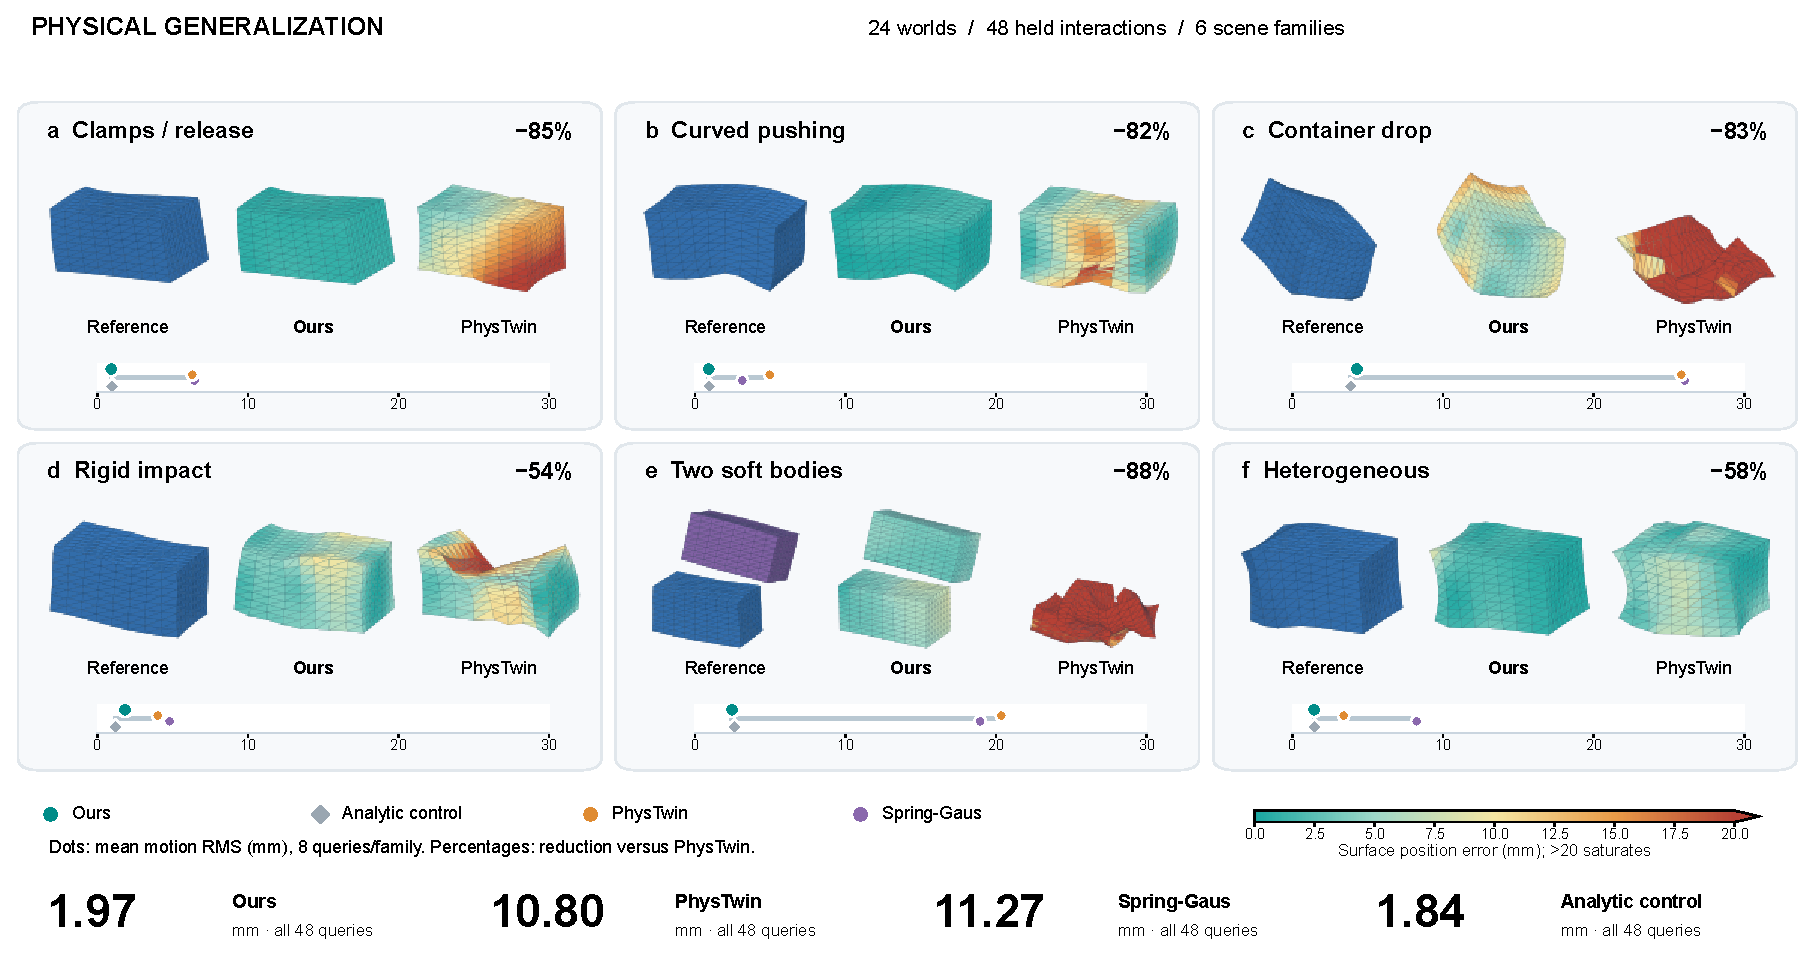
\includegraphics[width=.96\textwidth]{figures/sim-held_visual_results.pdf}
\caption{\textbf{Physical prediction across six interaction families.} Each panel shows the first world, query 0, final frame; error colors share a 0--20\,mm scale. Dots use all eight queries per family; percentages report mean-error reduction versus PhysTwin. The footer reports all 48 queries. Ours has lower mean error than both native spring adaptations in every family; the analytic control remains competitive. The supplement shows every comparator and the earlier drop cohort.}
\label{sim-fig:held-visual}
\end{figure*}

\clearpage
\onecolumn
\section{Spatial error maps across all six scene families}
\begin{figure}[ht]
\centering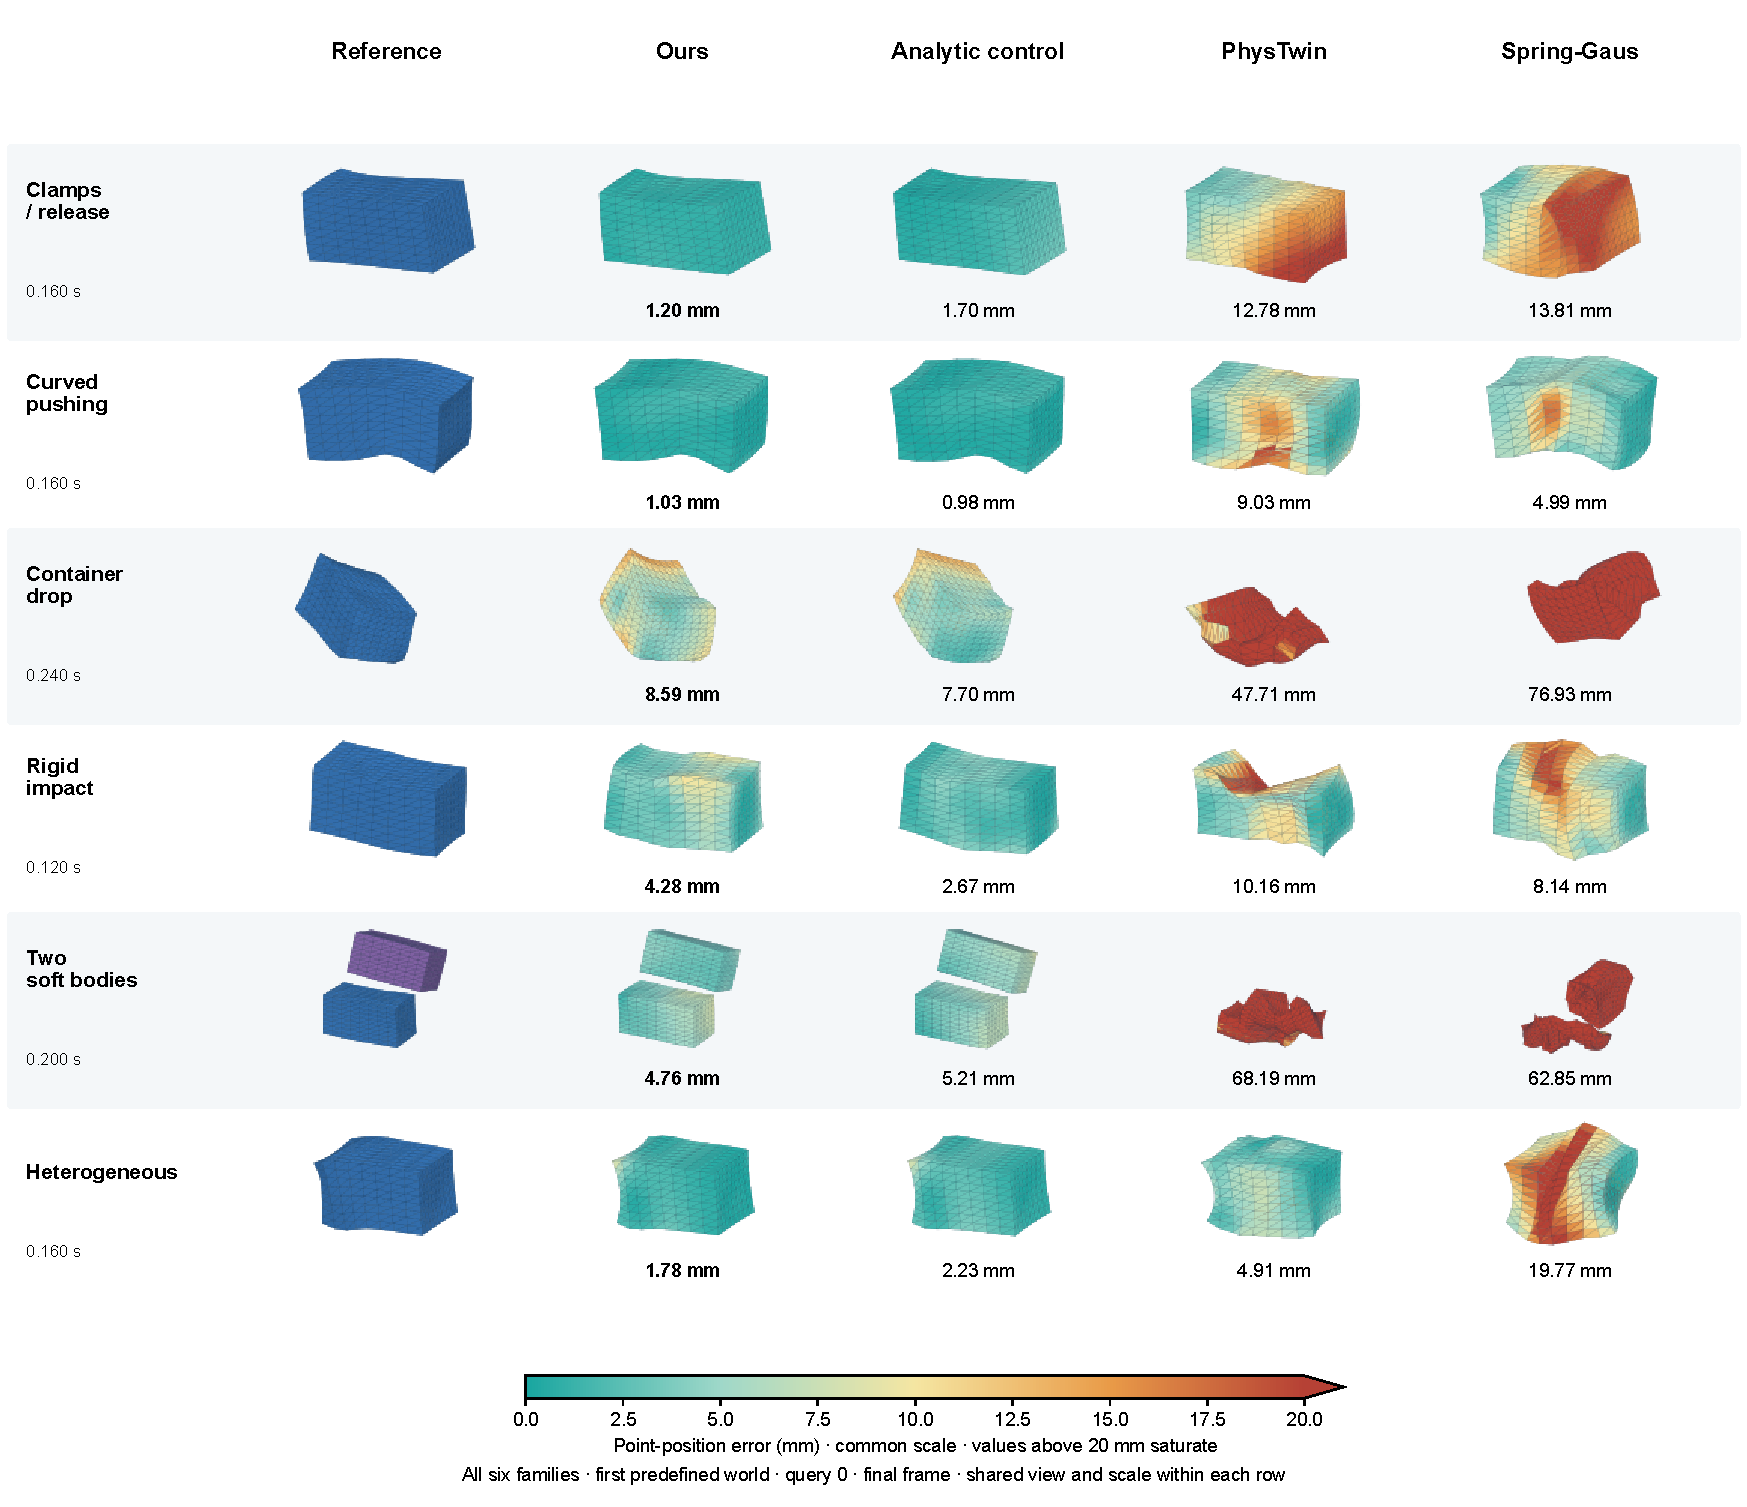
\includegraphics[width=.96\textwidth,height=.74\textheight,keepaspectratio]{figures/sim-held_error_plate.pdf}
\caption{\textbf{Where the predictions differ from the reference.} Every family uses its first predefined world, query 0 and final frame, without outcome-based selection. The numbers are point-vector RMS for that frame, not full-trajectory averages. All prediction surfaces use one 0--20\,mm point-error scale; triangle colors average vertex errors and larger values saturate. Camera and spatial bounds are shared within each row; deformation is not amplified. Reference surfaces use a solid body color. This geometry diagnostic is separate from Gaussian image-quality evaluation. UniPhy is unsupported in five families and fails on this selected drop query; it has no completed surface to plot here.}
\label{sim-fig:held-error-map}
\end{figure}
\clearpage
\twocolumn


\clearpage
\twocolumn
\part*{External Datasets and Real Interactions}

\section{Reading the Evidence}
This part records all per-sequence real-data results, all five declared transfer pairs, and all 40 fresh SoftVT episodes. It distinguishes the benchmark adapters used in the main paper from older exploratory variants. No prediction is refitted, selected per future outcome, or modified for this manuscript. The historical SoftVT illustration selected the largest improvement; the new main-paper teaser instead uses fixed declared simulation cases. Benchmark means retain every episode.

This external-dataset section studies two implementations of the material/interaction separation. The controlled simulator is specified in the preceding part. SoftVT's release model uses an analytic mechanics anchor with empirical correction. PhysTwin's current external adapter uses a frozen neural constitutive energy. There is no claim that the SoftVT gain was obtained with the neural decoder, nor that one shared checkpoint was trained across these datasets. The recent video-query reconstruction prototype is outside this work.

\section{Implementation Details}
\subsection{Initial geometry and material field}
The arbitrary-cloud FEM normalizes coordinates by the maximum initial bounding-box extent. A Delaunay tetrahedralization supplies elements; a support-distance filter removes elements bridging empty regions in nonconvex objects. The filter probes element centers and six edge midpoints, retaining probes within 0.045 normalized units of the initial support cloud. Elements with nearly zero reference determinant are excluded.

Six material kernels are selected from initial nodes by farthest-point sampling. Gaussian kernel values at element centers are normalized and volume-centered. The learned spatial scale is a linear combination of these features. Material coefficients are fitted within declared bounds. This compact field is an effective representation of the reconstructed object, not a measurement of six independently identified physical materials.

The analytic model uses Poisson ratio 0.35. The real neural adapter uses the pretrained scalar energy and a separate bounded volumetric adjustment,
\begin{equation}
\widetilde W=W_\theta+(e^\beta-1)e^s c_v(h,f)(J-\log J-1),
\end{equation}
where $c_v$ is the positive volumetric coefficient in the normalized pretrained law. The adjustment is zero at $\beta=0$. Decoder weights are never optimized on the real evaluation sequence.

\subsection{Pose and residual corrections}
The inherited SoftVT pipeline distinguishes rigid pose correction from a nonrigid empirical residual. A Kabsch alignment fits the discrepancy between the mechanics anchor and the permitted observed prefix. This discrepancy is expressed in the moving controller frame and transported to subsequent attached configurations.

For the residual candidate, a normalized feature vector combines controller-relative translation and rotated gravity. Ridge regression predicts local observed-point residuals from these features. Each marker's predicted residual magnitude is capped at twice its largest prefix residual, with a small positive floor. Inverse-distance interpolation over up to six initial observed neighbors transfers residuals to mechanical nodes. A finite rigid-alignment projection removes the rigid component before applying the nonrigid correction.

The historical selector compares no correction, pose correction and residual correction with strengths 0.25, 0.5 and 1.0. Its chronological validation uses the first 70\% of the available observation prefix for a separately fitted mechanics prediction and the remaining prefix for selection. Recalibration of the shortened input recomputes grasp geometry, so later validation observations do not define the fitted subprefix's attachment transform. The selected configuration is then refitted to the full permitted prefix. These corrections are empirical prediction devices, not inferred forces or constitutive laws.

The slip-aware experiment uses the frozen original mechanics/contact anchor, not a hindsight combination of whichever historical selector won a test sequence. Its eight-frame gravity-projected relative velocity and overlap threshold are fixed before the fresh 40-episode evaluation.

\subsection{Reduced contact rollout}
After release, node positions define a rigid body's instantaneous point distribution. The integrator updates translation and orientation under gravity and sequential static-surface impulses using ten substeps. The friction coefficient is 0.5 and restitution is zero. A position projection removes residual vertical penetration. Elastic shape and collision impulses are not jointly optimized. Consequently a successful placement prediction does not demonstrate accurate compression, friction coefficients or contact stress.

\subsection{Real-data solver settings and recovery}
The corrected real-data recipe uses 240 nodes, 18 prefix fitting frames and at most 50 parameter-optimization iterations, with a 1,800-second fitting budget and a 3,600-second total run budget. The ordinary equilibrium solve allows 80 iterations. One single-lift-zebra neural rollout frame exhausted that allowance; a recorded recovery retried the unchanged warm-start state and parameters with 320 iterations. It converged in 102 iterations with residual $1.36\times10^{-11}$ and minimum element determinant 0.714. No parameters were refitted for that recovery.

\section{Metrics and Aggregation}
For a frame containing $N$ nodes, coordinate RMSE is
\begin{equation}
E_{\mathrm{coord}}(t)=\sqrt{\frac1{3N}\sum_{i=1}^N\|\hat x_i(t)-x_i(t)\|^2}.
\end{equation}
SoftVT reports the mean of these frame errors, then averages episodes equally. It is not the same quantity as a pooled RMS over all frames. Rigid-aligned shape error applies one best-fitting proper rigid transform per frame before scoring.

Real manual-track error averages pointwise Euclidean distances over finite annotations in each frame and then averages frames and sequences equally. Displacement error uses $\hat x_i(t)-\hat x_i(0)$ and $x_i(t)-x_i(0)$. Pair-distance-change error averages
\begin{equation}
\left|\big(\|\hat x_i^t-\hat x_j^t\|-\|\hat x_i^0-\hat x_j^0\|\big)-\big(\|x_i^t-x_j^t\|-\|x_i^0-x_j^0\|\big)\right|
\end{equation}
over unordered annotated pairs. All three errors are geometric. Missing annotations are excluded; missing predictions are failures, not zero errors. Real transfer scores every noninitial target frame; sequence continuation uses the released test suffix.

\paragraph{Image metrics.}
A fixed crop comes from the reference foreground mask plus eight pixels of padding. Background treatment is common to all methods, and predicted spill within the crop remains penalized. PSNR uses RGB mean squared error, SSIM uses the common crop, and LPIPS uses a frozen perceptual network. Three noninitial times and three cameras produce nine images per sequence and 72 per method. Frame zero is excluded from the reported means. No image metric is reported for arbitrary unrecorded cameras because no reference RGB exists there.

\begin{table*}[!t]
\centering\small\setlength{\tabcolsep}{3pt}
\caption{All eight corrected-mask real sequence continuations. Mean manual-track distance in mm, lower is better. Each method completes all eight sequences. These historically exposed sequences are an exploratory benchmark, not a sealed new-object test.}
\begin{tabular}{lrrrr}\toprule
Sequence & Ours, neural & Analytic & Position ridge & Released PhysTwin\\\midrule
single\_lift\_sloth & 38.17 & 37.57 & 47.61 & 24.93\\
single\_lift\_dinosor & 47.08 & 52.79 & 17.80 & 16.63\\
single\_push\_sloth & 62.13 & 60.90 & 36.62 & 21.12\\
double\_lift\_sloth & 34.11 & 34.99 & 29.32 & 28.13\\
double\_stretch\_sloth & 16.01 & 15.17 & 7.89 & 9.75\\
single\_lift\_zebra & 62.13 & 69.15 & 46.61 & 24.30\\
double\_lift\_zebra & 34.43 & 32.07 & 25.64 & 31.20\\
double\_stretch\_zebra & 18.04 & 21.66 & 20.84 & 13.08\\
\midrule Equal-sequence mean &39.01&40.54&29.04&21.14\\\bottomrule
\end{tabular}
\end{table*}
\begin{table*}[!t]
\centering\small\setlength{\tabcolsep}{3pt}\setlength{\tabcolsep}{4pt}
\caption{All five declared real transfer pairs, including failed initial-geometry gates. Values are full noninitial interaction tracking errors in mm. Only the two passing pairs enter the primary transfer mean.}
\begin{tabular}{llcrrrr}\toprule
Source & Target & Gate & Ours & Analytic & Frozen native & Persistence\\\midrule
single\_lift\_sloth & double\_lift\_sloth & Fail & 21.50 & 21.71 & 58.97 & 57.77\\
single\_lift\_sloth & double\_stretch\_sloth & Fail & 31.87 & 33.07 & 42.36 & 38.37\\
single\_lift\_sloth & single\_push\_sloth & Pass & 42.78 & 42.73 & 58.23 & 112.55\\
single\_lift\_zebra & double\_lift\_zebra & Pass & 35.54 & 39.06 & 31.02 & 45.68\\
single\_lift\_zebra & double\_stretch\_zebra & Fail & 39.76 & 43.54 & 39.50 & 46.24\\
\midrule\multicolumn{3}{l}{Two passing pairs} &39.16&40.90&44.63&79.11\\
\multicolumn{3}{l}{All five, diagnostic only} &34.29&36.02&46.02&60.12\\\bottomrule
\end{tabular}
\end{table*}
\section{Real-Data Protocol and Historical Results}
\paragraph{Ordinary continuation.}
The eight-sequence table retains sloth, zebra and dinosaur sequences without choosing a subset where the new adapter wins. The released PhysTwin forecast is the comparator, not a retrained model with an artificially restricted fitting budget. Our 240-node neural and analytic adapters use the same external geometry recipe and prefix input contract. Differences in the physical forecasts include discretization, fitting budget and dynamics. Our image evaluation applies a common appearance transport to those forecasts; it is not a comparison of separately optimized native rendering pipelines.

\paragraph{Frozen transfer.}
The compatibility test is fixed before target-motion scoring: symmetric median initial registration distance must be below 3\% of the source bounding-box diagonal, and the 95th percentile below 8\%. Sloth lift-to-push and zebra one-hand-to-two-hand lift pass. The three other pairs remain in the diagnostic table, rather than being silently dropped. Identity follows the release's object names; independent confirmation of material identity and rest-state compatibility is not available.

The native frozen adaptation preserves source object springs, reconstructs target controller connections geometrically and assigns the median source controller stiffness to the new connections. Our adapter uses the registered source material field and median source attachment strength. Neither fits target motion after initialization. Initial manual-track matching is common across methods and can itself contribute an offset; this motivates reporting displacement and pair-distance-change metrics alongside absolute tracking.

\paragraph{Preserving the earlier best benchmark results.}
The development archive contains an earlier selected PhysTwin predictor with mean manual error 33.019\,mm, stronger than subsequent 41.277\,mm attachment-width and 43.104\,mm Gaussian-residual variants. A guarded ridge-switch extension gave 37.044\,mm and was not promoted. These values are retained below as historical results, not relabeled as outputs of the current neural model.

\begin{table}[h]
\centering\small\setlength{\tabcolsep}{3pt}
\caption{Historical PhysTwin configurations on eight exposed sequences. Old input/export and selection protocols; these are not a matched ablation against the corrected-mask table above.}
\begin{tabular}{lr}\toprule
Archived configuration & Track error (mm)\\\midrule
Prior selected predictor &33.019\\
Guarded ridge-switch extension &37.044\\
Attachment-width primary &41.277\\
Always-on Gaussian residual &43.104\\
Original mechanics/contact anchor &43.426\\\bottomrule
\end{tabular}
\end{table}

The old adapter used different masks, geometry and correction rules. In the current corrected export, a position at time $t$ uses incoming transition validity from $t-1$, rather than the outgoing transition from $t$ to $t+1$. We do not compare historical scores as though only one architectural component changed. The primary manuscript uses the corrected-mask neural and analytic records and gives the historical best its own provenance.



\clearpage
\onecolumn
\section{All Fresh SoftVT Episodes}
\begin{center}
\small
\begin{tabular}{lrrr}\toprule
Episode & Original mechanics/contact (mm) & Ours with slip (mm) & Improvement (mm)\\\midrule
object-soft-task1-demo40 & 16.031 & 15.868 & +0.163\\
spatial-soft-task1-demo40 & 12.417 & 10.148 & +2.269\\
object-soft-task2-demo40 & 12.967 & 12.864 & +0.103\\
spatial-soft-task2-demo40 & 54.241 & 52.756 & +1.485\\
object-soft-task1-demo41 & 16.559 & 16.134 & +0.425\\
spatial-soft-task1-demo41 & 12.579 & 10.170 & +2.409\\
object-soft-task2-demo41 & 13.308 & 13.458 & -0.150\\
spatial-soft-task2-demo41 & 22.623 & 17.402 & +5.221\\
object-soft-task1-demo42 & 16.702 & 16.484 & +0.218\\
spatial-soft-task1-demo42 & 11.770 & 10.384 & +1.386\\
object-soft-task2-demo42 & 13.329 & 13.130 & +0.199\\
spatial-soft-task2-demo42 & 34.385 & 33.711 & +0.674\\
object-soft-task1-demo43 & 16.283 & 15.996 & +0.287\\
spatial-soft-task1-demo43 & 11.082 & 10.194 & +0.887\\
object-soft-task2-demo43 & 13.246 & 13.149 & +0.098\\
spatial-soft-task2-demo43 & 19.793 & 16.415 & +3.378\\
object-soft-task1-demo44 & 15.649 & 15.465 & +0.185\\
spatial-soft-task1-demo44 & 12.240 & 10.044 & +2.196\\
object-soft-task2-demo44 & 12.697 & 12.903 & -0.206\\
spatial-soft-task2-demo44 & 56.061 & 54.759 & +1.302\\
object-soft-task1-demo45 & 17.165 & 16.795 & +0.371\\
spatial-soft-task1-demo45 & 12.437 & 9.369 & +3.068\\
object-soft-task2-demo45 & 13.637 & 13.606 & +0.031\\
spatial-soft-task2-demo45 & 18.151 & 15.140 & +3.011\\
object-soft-task1-demo46 & 15.687 & 14.907 & +0.781\\
spatial-soft-task1-demo46 & 11.847 & 10.493 & +1.354\\
object-soft-task2-demo46 & 11.753 & 11.662 & +0.091\\
spatial-soft-task2-demo46 & 16.481 & 13.610 & +2.871\\
object-soft-task1-demo47 & 17.194 & 16.797 & +0.398\\
spatial-soft-task1-demo47 & 12.460 & 10.403 & +2.057\\
object-soft-task2-demo47 & 12.976 & 12.926 & +0.049\\
spatial-soft-task2-demo47 & 58.251 & 57.654 & +0.597\\
object-soft-task1-demo48 & 34.294 & 35.380 & -1.086\\
spatial-soft-task1-demo48 & 13.020 & 10.851 & +2.169\\
object-soft-task2-demo48 & 12.922 & 13.154 & -0.232\\
spatial-soft-task2-demo48 & 21.727 & 20.391 & +1.336\\
object-soft-task1-demo49 & 15.707 & 15.351 & +0.356\\
spatial-soft-task1-demo49 & 12.651 & 10.698 & +1.953\\
object-soft-task2-demo49 & 13.140 & 13.122 & +0.018\\
spatial-soft-task2-demo49 & 21.828 & 20.851 & +0.977\\
\midrule Equal-episode mean &18.932&17.865&+1.067\\\bottomrule
\end{tabular}
\end{center}
\noindent All 40 episodes and all 1,998 forecast frames are complete. Positive improvement favors ours. The four losses remain in the mean. Episode IDs 40--49 are drawn from two tasks in each of the object-soft and spatial-soft suites. These are repeated-asset episodes, not 40 distinct objects. The reported bootstrap resamples paired episodes and therefore describes this episode cohort, not unseen-object uncertainty.

\clearpage
\twocolumn
\section{Regression Preservation and Supporting Studies}
\paragraph{SoftVT regression inventory.}
The full inventory contains 220 cases across development, historical and prospective cohorts. The robust predictor completes all 220 trajectories. The numerical fallback is triggered only by a nonfinite original nodal trajectory, repairing object-soft-task2-demo31. All 179 previously finite Phase A predictions remain bitwise identical. The earlier 40 confirmation episodes include an original trajectory with missing frames; their available-frame baseline mean must not be treated as a complete paired forecast score. The main paper instead uses the later fresh 40-episode cohort where both methods have complete coverage.

\section{Figure Provenance and Reproduction}
Figures are generated programmatically from saved data and metrics. The historical SoftVT illustration uses spatial-soft-task2-demo41, the largest improvement among the 40 fresh episodes; it is not the new main-paper teaser. Its timestamp is 75\% through the forecast suffix. Surface triangles come from the initial node convex hull solely for visualization, and the saved node positions are unchanged. The reference and predictions share world limits and camera. No deformation amplification or separate per-method alignment is applied.

The real image panel uses the first declared continuation sequence, single-lift sloth, at final frame 84 in camera 2. Any newly assembled panels retain their own selection records in the figure manifest. The new main-paper panel uses one common reference-mask crop; the archived panel displayed full images. Its appearance assets and transport policy are shared across methods. The method diagram is a schematic of coordinate roles, not generated experimental evidence. Scatter plots and bars include complete declared cohorts.

The editable source package includes precomputed vector PDF figures, so it can compile without raw datasets. Figure regeneration requires the original benchmark assets and saved predictions. A provenance manifest records the exact evaluation sources, hashes and selection rules. The original benchmark records remain unchanged. The paper build performs table checks and verifies numerical summaries without launching fitting or simulation jobs.

\paragraph{Claim boundaries.}
The work does not claim overall state-of-the-art performance on either dataset's native task, learned camera estimation, image-only material recovery, force accuracy from real captures, calibrated uncertainty, or superiority of uncertainty-guided probing. The external evidence provides a complete prospective episode test, a corrected real continuation benchmark and a limited cross-interaction transfer pilot, complementing the controlled mechanics results above. These are the claims supported by the reported artifacts.

\section{Later Conditional-Flow Diagnostics}
The following expansion is a separate experiment rather than a replacement for the main-paper predictors. Spatial Gaussian-boundary models use a 128-accepted-bank/256-attempt budget, 5,000 training steps and 32 posterior draws, with matched flow and mixture models and nearest-bank controls. The observation budget and geometry differ from the earlier external studies. These scores must not be substituted into their tables.

\paragraph{Prospective SoftVT cohort.}
Twelve declared cases use two suites, tasks 0--2 and episodes 50--51. Eleven physics pipelines complete; object-soft/task 1/demo 50 fails bank admission under its fixed budget. Standalone persistence, velocity and rigid/contact controls complete all twelve. On the common eleven, flow-contact coordinate/shape errors are 19.245/1.743\,mm versus 19.054/1.199\,mm for rigid/contact and 19.512/2.122\,mm for nearest-bank contact. Flow improves retrieval slightly, not the stronger rigid control. Of 352 flow draws, 342 produce valid trajectories and ten fail; failure counts remain visible.

\paragraph{Eight real plush cases.}
All eight physics cases complete under the separate compact-geometry protocol. Flow-contact coordinate/shape errors are 37.242/19.790\,mm, rigid/contact 39.776/24.635\,mm, nearest-contact 37.024/18.932\,mm and nearest-raw 30.794/18.932\,mm. These forecast-observable scores are not the manual-track metric used by the main corrected-mask real table. Stretching improves aligned shape relative to rigid motion by roughly 25\% and 46\%, but nearest retrieval remains better. Four of 256 flow draws fail.

\paragraph{Calibration.}
Nominal 90\% marginal coordinate intervals cover 7.02\% on SoftVT and 9.15\% on PhysTwin for flow-contact, conditional on successful physics cases and surviving draws. The contact/pose operation does not preserve a calibrated posterior. Coverage therefore cannot justify uncertainty-guided intervention. The earlier static additional-observation study has a related warning: improved point estimates coexist with poorer interval coverage.

\paragraph{Separate RGB-D bridge.}
A different conditional flow predicts a restricted global 25-dimensional physical code and four-way boundary/force categories from five RGB-D observations. It is not the spatial Gaussian field. Training/validation use 152/44 episodes; 76 previously exposed Isaac episodes provide retrospective recorded-motion evaluation. Five methods complete 380 method-case predictions before target scoring. Position error is 0.754\,mm for flow, 0.736 for matched mixture density, 0.694 for an archived 25D predictor, 0.730 for a chart model and 0.717 for ridge. An explicitly retrospective static control yields 0.732\,mm and all five models lose to static on mean aligned-shape error. These small-motion, zero-gravity episodes do not establish accurate impact physics.

\paragraph{Bounded follow-up and adoption.}
A fixed best/final checkpoint comparison on 44 recorded validation cases produces 176 forecasts. Selecting the final flow checkpoint improves coordinate error by only 0.46\% while worsening shape and parameter coverage; no new test rerun or global replacement follows. A known-parameter roundtrip uses two training-bank worlds, not new generalization tests, and retains seven failed rollouts. A no-contact elastic-continuation prototype remains qualified only on its small refinement fixture. The prior best predictors and main-paper results are preserved.

\paragraph{Dataset coverage.}
Fourteen additional PhysTwin cloth/rope/composite sequences are unsupported by the present volumetric adapter. PokeFlex recordings are not available under approved access, and Deform360 evaluation is deferred. Inventory is not execution; neither dataset is claimed as a completed benchmark here.

\section{Artifact and Review Checklist}
The source package includes self-contained PDF figures, all manuscript sources and the official unmodified style. Evidence manifests record the local numerical sources and their hashes without bundling raw captures, checkpoints or large trajectories. Scripts regenerate plots from those artifacts. Different metric definitions, observation budgets, known boundaries, failures and retrospective analyses remain explicit.

No submission identifier or author identity is fabricated. The manuscript and supplement require author approval and registration before submission. Anonymous review PDFs contain no identifying repository link or external content needed to understand the results. Additional media illustrate saved trajectories and are not additional independent trials.

\clearpage
\onecolumn
\section{Additional Visual Comparisons}
The main paper highlights selected successful public-dataset predictions. The following figures retain aggregate context and a real continuation case where the native model is stronger. The public-dataset zooms use identical recorded images or unaltered simulation nodes, matched crops and explicit error annotations; no image synthesis or geometric exaggeration is used. The selected real landmark improves from 206.1 to 31.6\,mm; the selected SoftVT material point improves from 18.5 to 13.6\,mm. They are local illustrations, not aggregate benchmark scores.
\begin{center}
\centering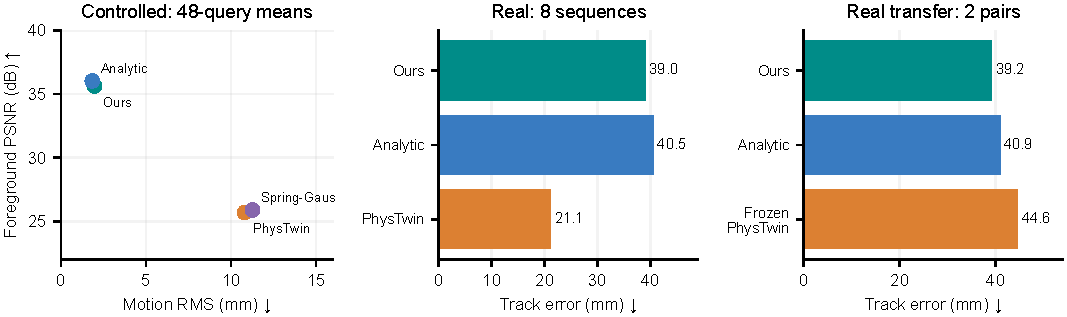
\includegraphics[width=\textwidth]{figures/cohesive-outcomes.pdf}
\captionof{figure}{\textbf{Physical and image agreement under explicit protocols.} Left: method means over the same 48 controlled queries, with fixed appearance and transport, expose motion-induced image error; this is numerical-reference agreement, not measured real-world material accuracy. Right: released PhysTwin wins the eight real continuations, while our frozen adapter has a lower mean on the two qualified changed interactions. These are different tasks and metric definitions; no cross-panel average is formed.}
\label{fig:outcomes}
\end{center}
\begin{center}
\centering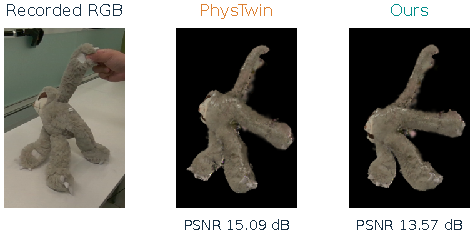
\includegraphics[width=.48\textwidth]{figures/cohesive-real-capture.pdf}
\captionof{figure}{\textbf{A real continuation failure.} First declared sloth-lift sequence, final frame, camera 2; identical reference-derived crop. Both predictions use the same initial Gaussian appearance. PhysTwin follows the captured object more closely here, consistent with its advantage on the complete continuation cohort.}
\label{fig:realcapture}
\end{center}
\clearpage
\section{Earlier Coarse Equilibrium Adapter on PIDG}
\label{sec:pidg-rendering}
This earlier diagnostic separates appearance initialization from hard mechanical coupling; it is distinct from the dense soft-constrained hybrid above. It uses the public synthetic \emph{Balls Reaction} scene of PIDG~\cite{hong2026pidg}. It is an equilibrium reconstruction adapter, not the transient coupled-contact experiment in the main paper. It does not establish material identification from RGB, causal prediction of a new action, or quantitative accuracy at unrecorded cameras.

\paragraph{Observed inputs and physical hypotheses.}
We retain the declared 101 fitting, 11 validation and 38 test images, with supplied camera poses and a common frame-index clock. A fitting-only PIDG reconstruction initializes the radius/depth gauge. Connected color regions in the fitting images supply object-position and apparent-shape observations. Six separately represented, approximately spherical objects are an explicit initialization prior. Each object has 13 mechanical nodes, 20 tetrahedra and six localized Gaussian attachment footprints. The attachment targets are inferred position controls, not observed real grippers. The shared learned material decoder is frozen. Material descriptors are inherited from the initial image/mechanics fit and held fixed during the appearance-transfer refinement. Gravity is negligible under the unidentified physical scale, and this adapter does not solve coupled inter-object collisions.

\paragraph{Connected inference and rendering.}
For physical parameters $\eta$ and inferred boundary targets $b$, equilibrium satisfies $r(x;\eta,b)=0$. Differentiating an image loss $L$ uses
\begin{equation}
 H^\top\lambda=\frac{\partial L}{\partial x},\qquad
 \frac{dL}{d(\eta,b)}=-\lambda^\top\frac{\partial r}{\partial(\eta,b)},\quad H=\frac{\partial r}{\partial x}.
\end{equation}
The renderer therefore updates a solved physical state rather than an unconstrained deformation MLP. All 228 held-image object equilibria converge with residual below $9.73\times10^{-8}$; the minimum tetrahedral Jacobian is 0.868. These numerical checks do not establish correct contact or material identification. Gaussian centers use fixed material-coordinate bindings, covariance follows $\Sigma_t=F_t\Sigma_0F_t^\top$, and view directions are pulled into the material rotation frame for spherical-harmonic radiance. The boundary adjoint agrees with finite differences, and the binding passes affine-position and covariance tests. The earlier sparse-appearance adapter used 4,608 newly initialized Gaussians and achieved only 25.59\,dB test PSNR at $320\times180$ despite converged mechanical states. This motivates retaining fitted appearance instead of conflating its initialization error with a constitutive-model comparison.

\paragraph{Appearance-preserving reference binding.}
We transfer all 50,524 fitted Gaussian centers, full covariances, opacities and spherical-harmonic coefficients from the matched local PIDG reconstruction at the first fitting frame. At the renderer-conversion stage, RGB RMSE against the original render is $1.55\times10^{-8}$ and both renders have 56.33\,dB PSNR on that fitting image. This is a conversion check, not a test-set result. The covariance calculation matches the released rasterizer's unnormalized-quaternion convention; silently normalizing those quaternions changes the image. Material bindings use the physical state at that reference frame, including explicitly disclosed affine extrapolation outside the coarse tetrahedral mesh. Fitted appearance does not supply ground-truth hidden geometry.

\paragraph{Selection and interpretation.}
Appearance refinement and boundary refinement use only fitting RGB. Temporal controls include global pose/scale and six independently translated Gaussian boundary patches per object; joint fitting is followed by appearance-only refinement with mechanics fixed. Checkpoint selection uses validation foreground PSNR. A validation-only radiance ablation favors material-frame over world-frame directions. All candidate runs are retained. A checkpoint audit found that appearance-only regularization had changed controls behind cached geometry. Restoring the exact controls used to build that cache recovers identical live validation scores; the corrected optimizer freezes those controls explicitly. The invalid evaluation is retained in the artifact audit and excluded from the reported table. Canonical Gaussian offsets and covariance-scale corrections are bounded. PIDG is used for appearance initialization, so this is a reconstruction-assisted comparison rather than an independently initialized competitor. This released test split has also been evaluated in earlier development; it is not a newly collected confirmatory cohort. All methods are trained at $320\times180$; rendering at a larger resolution is not retraining at that resolution. The original paper's 33.31\,dB Balls Reaction score is reported under a different training setup and is not substituted for our matched baseline.

\paragraph{Measured reconstruction results.}
Table~\ref{tab:pidg-rendering} reports all 38 test images. Transferring appearance and refining boundary targets improves the connected model, while the unconstrained PIDG reconstruction remains stronger on recorded cameras. Larger output images use the same $320\times180$ training. These are held-image reconstruction scores, not forecasts of a new force.
\begin{center}
\captionof{table}{\textbf{PIDG Balls Reaction, matched image split.} Full-image / foreground PSNR (dB; higher is better), SSIM (higher) and AlexNet LPIPS (lower). The transferred model uses PIDG appearance initialization.}
\label{tab:pidg-rendering}
\begin{tabular}{llrrrr}
\toprule Output width & Method & PSNR & FG PSNR & SSIM & LPIPS \\
\midrule
320 & PIDG & 49.54 & 39.62 & 0.9987 & 0.0004 \\
320 & Ours: coarse appearance & 25.59 & 19.81 & 0.9210 & 0.0827 \\
320 & Ours: transferred appearance & 31.43 & 22.89 & 0.9710 & 0.0245 \\
\midrule
640 & PIDG & 34.48 & 25.28 & 0.9845 & 0.0086 \\
640 & Ours: coarse appearance & 25.50 & 19.28 & 0.9242 & 0.0823 \\
640 & Ours: transferred appearance & 29.86 & 20.83 & 0.9549 & 0.0442 \\
\midrule
1600 & PIDG & 31.64 & 22.41 & 0.9712 & 0.0323 \\
1600 & Ours: coarse appearance & 25.40 & 19.01 & 0.9335 & 0.0896 \\
1600 & Ours: transferred appearance & 28.68 & 19.35 & 0.9473 & 0.0662 \\
\bottomrule\end{tabular}\end{center}
\begin{center}\begin{minipage}{\textwidth}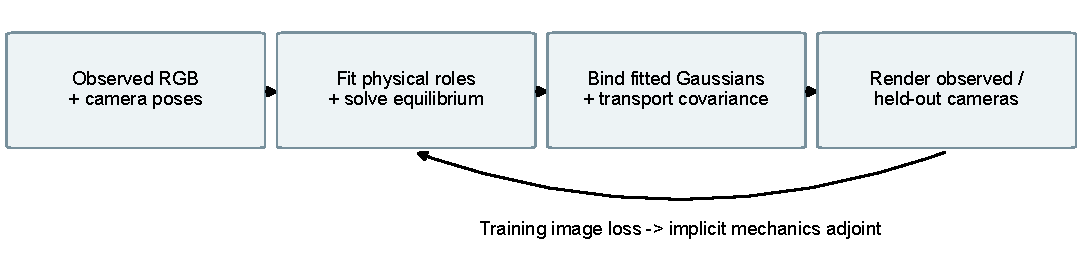
\includegraphics[width=\textwidth]{figures/pidg-rendering-loop.pdf}
\captionof{figure}{\textbf{Image loss reaches the physical state.} Boundary controls update solved equilibrium through an implicit adjoint. Appearance-only refinement then holds the selected mechanics fixed; query-time images use mechanics-transported Gaussians.}\end{minipage}\end{center}
\begin{center}\begin{minipage}{\textwidth}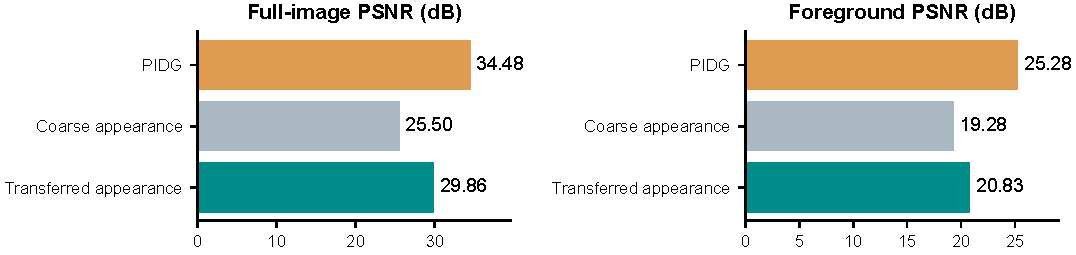
\includegraphics[width=\textwidth]{figures/pidg-rendering-metrics.pdf}
\captionof{figure}{\textbf{Aggregate recorded-camera reconstruction at width 640.} Foreground scores prevent the black background from dominating interpretation. Native PIDG remains ahead; the transferred mechanical renderer improves on its previous coarse initialization.}\end{minipage}\end{center}
\clearpage
\begin{center}\begin{minipage}{\textwidth}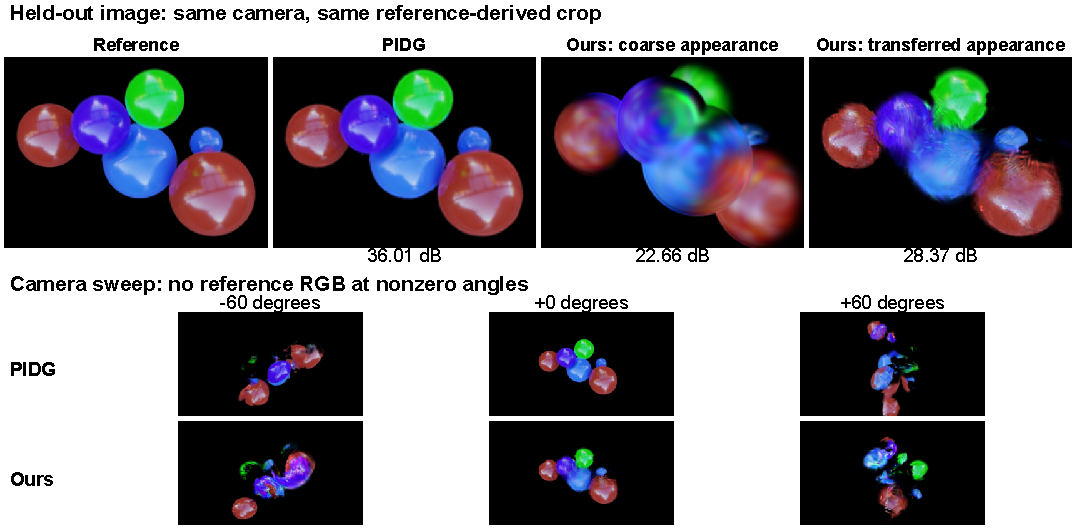
\includegraphics[width=\textwidth]{figures/pidg-rendering-comparison.pdf}
\captionof{figure}{\textbf{Appearance refinement and camera sweep.} The middle declared test time is fixed in advance. Top: identical reference-derived crop and per-frame full-image PSNR. Bottom: fixed camera offsets, with no reference RGB at nonzero angles. The spherical geometry prior contributes to coherence; these views do not prove hidden-surface accuracy or material identification.}\end{minipage}\end{center}


{\small\bibliographystyle{ieeenat_fullname}\bibliography{references}}
\end{document}
